\documentclass[11pt]{article}
\usepackage[margin=1in]{geometry}
\usepackage{amsmath,amssymb}
\usepackage{booktabs,longtable,array,graphicx,float}
\usepackage{xcolor}
\usepackage[hidelinks]{hyperref}
\usepackage{caption}
\captionsetup{font=small,labelfont=bf}
\setlength{\LTcapwidth}{\linewidth}
\title{Resource Costs of the Cosine-Filter Pipeline for the Open $J_1$--$J_2$ Chain\\[2pt]\large Results, with every quantity defined}
\author{}
\date{}
\begin{document}
\maketitle

\section{What this report shows}
A shallow circuit built from a DMRG state leaves some excited-state weight. A \emph{cosine filter} (the Stetcu--Baroni--Carlson projection) removes it using one extra qubit, controlled time evolution, and post-selection. This report gives the \textbf{gate cost of that filter} for the spin-$\tfrac12$ $J_1$--$J_2$ chain with $N$ up to 32, at the target error $\varepsilon=10^{-2}$ (and $10^{-1}$), together with the accuracy of the classical DMRG inputs and a check of every proven bound. Every symbol is defined in Section~\ref{sec:glossary}. The error guarantees are \emph{conditional certificates}: they hold if the DMRG energies and the trial-state weight are exact, which DMRG cannot itself certify (Section~\ref{sec:limits}); the derivation of every chosen value is in \texttt{CERTIFICATION.tex}.

\section{Headline results}
\begin{itemize}
\item \textbf{DMRG inputs are accurate.} Energies agree with exact diagonalisation to $3.7e-13$ ($N\leq20$); independent DMRG runs agree to $1.2e-13$ for $N=24$--$32$.
\item \textbf{Small chains ($N\leq14$, $\varepsilon=10^{-2}$).} Guaranteed designs need 76--24\,027 Trotter steps and 1\,539--3\,604\,089 RZZ gates; the measured error stays below the proven bound in all 60 simulated designs (violations: 0). The guaranteed design needs 15--586$\times$ the steps of the oracle design.
\item \textbf{Larger chains ($N=16$--$32$, $\varepsilon=10^{-2}$).} 16\,485--314\,923 steps, $2.4\times10^{6}$--$1.0\times10^{8}$ RZZ with block re-synthesis ($4.8\times10^{6}$--$2.0\times10^{8}$ RZZ with direct compilation) and $1.2\times10^{6}$--$5.0\times10^{7}$ non-Clifford rotations (direct compilation; $2.1\times10^{6}$--$8.4\times10^{7}$ with re-synthesis), with physical evolution time 7.9--20.5 (units of $1/J_1$). Total RZZ grows like $N^{5.1}$ ($J_2=0$, $N=6$--$24$), $N^{5.2}$ ($J_2=0.2411$, $N=6$--$28$), $N^{4.9}$ ($J_2=0.4$, $N=6$--$32$).
\item \textbf{The bandwidth does not change the cost.} Switching from the earlier Pauli-$\ell_1$ bandwidth to the Weyl bandwidth changed the guaranteed step count by a factor 0.63--1.14 (median 0.99) and the physical time by 0.67--1.50, over 59 matching designs.
\item \textbf{Limit.} For $N=28,32$ at $J_2=0$ and $0.2411$ the shallow trial circuit has too little ground-state weight, and no certified filter with at most 8 pulses reaches $\varepsilon=10^{-2}$ (Fig.~\ref{fig:gamma}).
\end{itemize}

\section{Glossary: every term used}\label{sec:glossary}
\begin{longtable}{p{0.2\linewidth}p{0.74\linewidth}}
\toprule
Term & Meaning \\
\midrule
\endhead
$N$ & number of spin-$\tfrac12$ sites in the open chain. \\
$J_1,J_2$ & nearest- and next-nearest-neighbour exchange couplings; $J_1=1$ sets the energy unit. $J_2=0.2411$ is one of the three values studied (the reference value of $J_{2,c}$ from the literature). \\
$H$ & Hamiltonian $H=J_1\sum_i\mathbf S_i\!\cdot\!\mathbf S_{i+1}+J_2\sum_i\mathbf S_i\!\cdot\!\mathbf S_{i+2}$, written as a sum of Pauli strings (``Pauli terms''). \\
$E_0,\,E_1,\,E_{\rm top}$ & lowest, second-lowest (first excited state of any symmetry) and highest energy of $H$. $g=E_1-E_0$ is the energy gap. \\
DMRG & density-matrix renormalisation group: a classical algorithm that finds low-energy states of 1D systems as matrix-product states (MPS). ``max bond'' is the largest MPS bond dimension reached. \\
$W$ & bandwidth, a rigorous upper bound on $E_{\rm top}-E_0$ obtained from Weyl's inequality (Section~\ref{sec:bandwidth}); here it equals $E_{\rm top}-E_0$. \\
$H_s,\ \Delta$ & scaled Hamiltonian $H_s=(H-E_0)/W$, whose ground state sits at $0$ and whose other levels lie in $[\Delta,1]$ with scaled gap $\Delta=g/W$. \\
trial state, $\gamma$ & the starting state prepared by a shallow circuit compiled from the DMRG state; $\gamma$ is its weight on the true ground state ($1-\gamma$ is the part the filter must remove). \\
filter $F(E)$ & $F(E)=\prod_{i=1}^m\cos(Et_i+\phi_i)$ with $m$ pulses of times $t_i$ and phases $\phi_i$; applied to the state it multiplies the weight of the energy-$E$ component by $F(E)$. \\
pulse, ancilla & one pulse is a Hadamard, a rotation, a controlled evolution $e^{-it_iH_s\otimes Z}$ and a Hadamard on one extra (ancilla) qubit; reading the ancilla as $0$ applies $\cos(H_st_i+\phi_i)$ to the system. The run is kept only if all ancilla readings are $0$ (post-selection). \\
$T,\ T_{\rm phys}$ & total evolution time $T=\sum_it_i$ in units of $1/W$; $T_{\rm phys}=T/W$ in units of $1/J_1$. \\
$\eta$ & certified ratio of the largest value of $|F|$ on $[\Delta,1]$ to $|F(0)|$: how strongly the filter suppresses excited states relative to the ground state. \\
$p_g$, $P_{\rm succ}$ & $p_g=\gamma F(0)^2$ is a proven lower bound on the success (post-selection) probability $P_{\rm succ}$; the expected number of repetitions is at most $1/p_g$. \\
$\varepsilon$, $1-F$ & target error: $1-F$ is the infidelity ($1$ minus the squared overlap) of the final state with the exact ground state; the design must prove $1-F\leq\varepsilon$. \\
Trotter steps $n$ & the controlled evolution is approximated by $n$ (in total, over all pulses) first-order product-formula steps; $k_i$ steps in pulse $i$, $t_i=k_i\,{\rm d}t$. \\
$\alpha$ & commutator constant $\alpha=\sum_g\|[H_g,\sum_{g'>g}H_{g'}]\|$ of the scaled Hamiltonian: it sets the Trotter error $\alpha T^2/(2n)$. \\
guaranteed design & smallest $n$ for which the \emph{proven} bound on $1-F$ is $\leq\varepsilon$ (needs no ground state). \\
empirical (oracle) design & smallest $n$ for which the \emph{measured} $1-F$ is $\leq\varepsilon$; requires simulation and the exact ground state, so it is a reference, only available for $N\leq14$. \\
RZZ, $R_z$, non-Clifford rotations, depth & two-qubit gates ${\rm RZZ}(\theta)=e^{-i\theta ZZ/2}$ (CX is not in the gate set; ${\rm RZZ}(\pi/2)$ is Clifford), single-qubit $z$-rotations, and circuit depth after transpiling to the basis $\{{\rm RZZ},R_z,\sqrt{X},X\}$. ``Non-Clifford rotations'' = $R_z$ plus RZZ gates whose angle is not a multiple of $\pi/2$: the expensive gates on fault-tolerant hardware. Clifford single-qubit gates are not tracked. \\
direct / level 3 & two compilations of the same circuit. \emph{Direct} (qiskit optimisation level 1): every ancilla-controlled Pauli rotation is a ladder of four Clifford RZZ($\pi/2$) around one $R_z$, giving $4\times$(Pauli terms) RZZ and (Pauli terms $+1$) non-Clifford rotations per Trotter step. \emph{Level 3}: blocks are re-synthesised, giving two RZZ per Pauli term (one of them a non-Clifford RZZ($\theta$)), i.e. half the RZZ count, plus some extra non-Clifford $R_z$. \\
all-to-all / line & qubit connectivity assumed in the transpile: every qubit couples to every other, or the qubits sit on a line (extra RZZ from routing). \\
conditional certificate & the proven bound holds if the DMRG inputs ($E_0$, $E_1$, $\gamma$) are exact; they cannot be certified by DMRG itself (see Section~\ref{sec:limits}). \\
\bottomrule
\end{longtable}


\section{How the numbers are produced}\label{sec:method}
For each chain $(N,J_2)$ the pipeline does the following; all steps use only DMRG and circuits (no ground-state knowledge) except where marked.
\begin{enumerate}
\item \textbf{DMRG} finds $E_0$ and the ground-state MPS; a second DMRG run finds $E_1$ as the lowest state orthogonal to it, whatever its symmetry (the symmetry of the first excitation is not assumed: exact diagonalization finds a triplet for every $J_2\in[0,1]$ on the grid, open chains $N=8$, 12, 16, 20; closest approach of the first excited singlet to the triplet shrinks with $N$, see \texttt{WRITEUP.md} Section~7).
\item \textbf{Scale} $H\to H_s=(H-E_0)/W$ so that the spectrum lies in $\{0\}\cup[\Delta,1]$ (Section~\ref{sec:bandwidth}).
\item \textbf{Trial circuit}: the MPS is compiled to a shallow brickwork circuit ($L=1$ layer); $\gamma$ is its overlap with the DMRG ground state (computed from an MPS simulation of the circuit for $N>14$).
\item \textbf{Design the filter}: choose $m\leq8$ pulses, times $t_i$ and phases $\phi_i$ that maximise $F(0)^2$ subject to a \emph{certified} bound $\eta\leq\eta_{\rm target}(\varepsilon,\gamma)$.
\item \textbf{Choose $n$}: the smallest number of Trotter steps for which the proven bound $1-F\leq\big(\sqrt{\bar\ell}+\alpha T^2/(2n\sqrt{p_g})\big)^2\leq\varepsilon$ holds, where $\bar\ell$ is the leakage of the exact filter. (\emph{Empirical} design: simulate and take the smallest $n$ that works.)
\item \textbf{Count}: transpile one Trotter step once, multiply by $n$, add the trial circuit; checked against a full transpile (Section~\ref{sec:checks}).
\end{enumerate}

\section{Case inputs}\label{sec:inputs}
Table~\ref{tab:inputs} lists, for each chain, the DMRG energies and the quantities derived from them. The gap shrinks like $1/N$, so $W/g$ and hence the filter time grow with $N$ (Fig.~\ref{fig:gap}). The trial-state weight $\gamma$ falls with $N$ for fixed circuit depth, most strongly at small $J_2$ (Fig.~\ref{fig:gamma}); $1-\gamma$ is the infidelity of the trial \emph{circuit}, not an error of DMRG.
{\small
\begin{longtable}{rrrrrrrrrrr}
\caption{Inputs to the filter for every case (DMRG values; $J_1=1$). Definitions in Section~\ref{sec:glossary}.}\label{tab:inputs}\\
\toprule
$N$ & $J_2$ & $E_0$ & $g=E_1-E_0$ & $W$ & $\Delta=g/W$ & $\gamma$ & $1-\gamma$ & $\alpha$ & Pauli terms & trial RZZ \\
\midrule
\endfirsthead
\toprule
$N$ & $J_2$ & $E_0$ & $g=E_1-E_0$ & $W$ & $\Delta=g/W$ & $\gamma$ & $1-\gamma$ & $\alpha$ & Pauli terms & trial RZZ \\
\midrule
\endhead
\bottomrule
\endfoot
4 & 0 & -1.616025 & 0.65892 & 2.366 & 0.27849 & 0.9553 & $4.47\times10^{-2}$ & 0.2679 & 9 & 9 \\
6 & 0 & -2.493577 & 0.49158 & 3.744 & 0.13131 & 0.8981 & $1.02\times10^{-1}$ & 0.2141 & 15 & 15 \\
8 & 0 & -3.374933 & 0.39269 & 5.125 & 0.07662 & 0.8371 & $1.63\times10^{-1}$ & 0.1713 & 21 & 21 \\
10 & 0 & -4.258035 & 0.32736 & 6.508 & 0.05030 & 0.7738 & $2.26\times10^{-1}$ & 0.1417 & 27 & 27 \\
12 & 0 & -5.142091 & 0.28094 & 7.892 & 0.03560 & 0.7170 & $2.83\times10^{-1}$ & 0.1204 & 33 & 33 \\
14 & 0 & -6.026725 & 0.24623 & 9.277 & 0.02654 & 0.6610 & $3.39\times10^{-1}$ & 0.1046 & 39 & 38 \\
16 & 0 & -6.911737 & 0.21928 & 10.662 & 0.02057 & 0.6056 & $3.94\times10^{-1}$ & 0.0924 & 45 & 45 \\
18 & 0 & -7.797011 & 0.19773 & 12.047 & 0.01641 & 0.5568 & $4.43\times10^{-1}$ & 0.0827 & 51 & 51 \\
20 & 0 & -8.682473 & 0.18009 & 13.432 & 0.01341 & 0.5139 & $4.86\times10^{-1}$ & 0.0748 & 57 & 57 \\
24 & 0 & -10.453786 & 0.15295 & 16.204 & 0.00944 & 0.4319 & $5.68\times10^{-1}$ & 0.0628 & 69 & 69 \\
28 & 0 & -12.225441 & 0.13302 & 18.975 & 0.00701 & 0.3653 & $6.35\times10^{-1}$ & 0.0542 & 81 & 81 \\
32 & 0 & -13.997316 & 0.11774 & 21.747 & 0.00541 & 0.3080 & $6.92\times10^{-1}$ & 0.0476 & 93 & 93 \\
4 & 0.2411 & -1.538741 & 0.66106 & 2.409 & 0.27438 & 0.9807 & $1.93\times10^{-2}$ & 0.3977 & 15 & 9 \\
6 & 0.2411 & -2.335347 & 0.48779 & 3.826 & 0.12748 & 0.9492 & $5.08\times10^{-2}$ & 0.3295 & 27 & 15 \\
8 & 0.2411 & -3.135001 & 0.38588 & 5.247 & 0.07355 & 0.9111 & $8.89\times10^{-2}$ & 0.2672 & 39 & 21 \\
10 & 0.2411 & -3.936128 & 0.31910 & 6.668 & 0.04785 & 0.8690 & $1.31\times10^{-1}$ & 0.2223 & 51 & 27 \\
12 & 0.2411 & -4.738077 & 0.27201 & 8.091 & 0.03362 & 0.8252 & $1.75\times10^{-1}$ & 0.1897 & 63 & 33 \\
14 & 0.2411 & -5.540531 & 0.23703 & 9.514 & 0.02491 & 0.7810 & $2.19\times10^{-1}$ & 0.1651 & 75 & 39 \\
16 & 0.2411 & -6.343316 & 0.21003 & 10.937 & 0.01920 & 0.7366 & $2.63\times10^{-1}$ & 0.1461 & 87 & 45 \\
18 & 0.2411 & -7.146332 & 0.18854 & 12.361 & 0.01525 & 0.6940 & $3.06\times10^{-1}$ & 0.1310 & 99 & 51 \\
20 & 0.2411 & -7.949515 & 0.17105 & 13.784 & 0.01241 & 0.6526 & $3.47\times10^{-1}$ & 0.1186 & 111 & 57 \\
24 & 0.2411 & -9.556221 & 0.14428 & 16.632 & 0.00867 & 0.5757 & $4.24\times10^{-1}$ & 0.0998 & 135 & 69 \\
28 & 0.2411 & -11.163230 & 0.12475 & 19.480 & 0.00640 & 0.5050 & $4.95\times10^{-1}$ & 0.0861 & 159 & 81 \\
32 & 0.2411 & -12.770432 & 0.10988 & 22.329 & 0.00492 & 0.4417 & $5.58\times10^{-1}$ & 0.0757 & 183 & 93 \\
4 & 0.4 & -1.506776 & 0.67368 & 2.457 & 0.27421 & 0.9959 & $4.06\times10^{-3}$ & 0.4708 & 15 & 9 \\
6 & 0.4 & -2.265535 & 0.50219 & 3.916 & 0.12825 & 0.9880 & $1.20\times10^{-2}$ & 0.3957 & 27 & 15 \\
8 & 0.4 & -3.025191 & 0.40371 & 5.375 & 0.07511 & 0.9770 & $2.30\times10^{-2}$ & 0.3229 & 39 & 21 \\
10 & 0.4 & -3.785289 & 0.34012 & 6.835 & 0.04976 & 0.9638 & $3.62\times10^{-2}$ & 0.2695 & 51 & 27 \\
12 & 0.4 & -4.545626 & 0.29559 & 8.296 & 0.03563 & 0.9490 & $5.10\times10^{-2}$ & 0.2303 & 63 & 33 \\
14 & 0.4 & -5.306103 & 0.26259 & 9.756 & 0.02692 & 0.9333 & $6.67\times10^{-2}$ & 0.2008 & 75 & 39 \\
16 & 0.4 & -6.066666 & 0.23711 & 11.217 & 0.02114 & 0.9170 & $8.30\times10^{-2}$ & 0.1778 & 87 & 45 \\
18 & 0.4 & -6.827284 & 0.21681 & 12.677 & 0.01710 & 0.9000 & $10.00\times10^{-2}$ & 0.1595 & 99 & 51 \\
20 & 0.4 & -7.587941 & 0.20024 & 14.138 & 0.01416 & 0.8833 & $1.17\times10^{-1}$ & 0.1446 & 111 & 57 \\
24 & 0.4 & -9.109325 & 0.17479 & 17.059 & 0.01025 & 0.8490 & $1.51\times10^{-1}$ & 0.1217 & 135 & 69 \\
28 & 0.4 & -10.630766 & 0.15613 & 19.981 & 0.00781 & 0.8153 & $1.85\times10^{-1}$ & 0.1051 & 159 & 81 \\
32 & 0.4 & -12.152237 & 0.14184 & 22.902 & 0.00619 & 0.7823 & $2.18\times10^{-1}$ & 0.0924 & 183 & 93 \\
\end{longtable}
}
\begin{figure}[htbp]
\centering
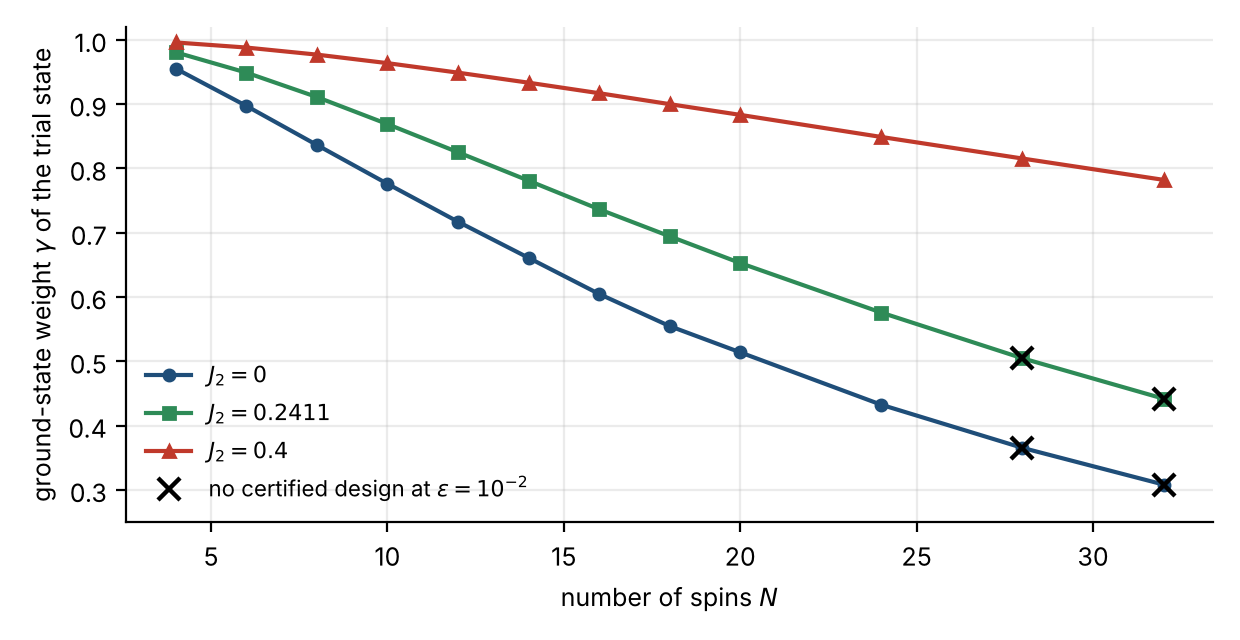
\includegraphics[width=0.75\linewidth]{figures_tex/gamma_vs_N.png}
\caption{Ground-state weight $\gamma$ of the $L=1$ trial circuit against $N$. Crosses mark cases where no certified filter reaches $\varepsilon=10^{-2}$.}\label{fig:gamma}
\end{figure}
\begin{figure}[htbp]
\centering
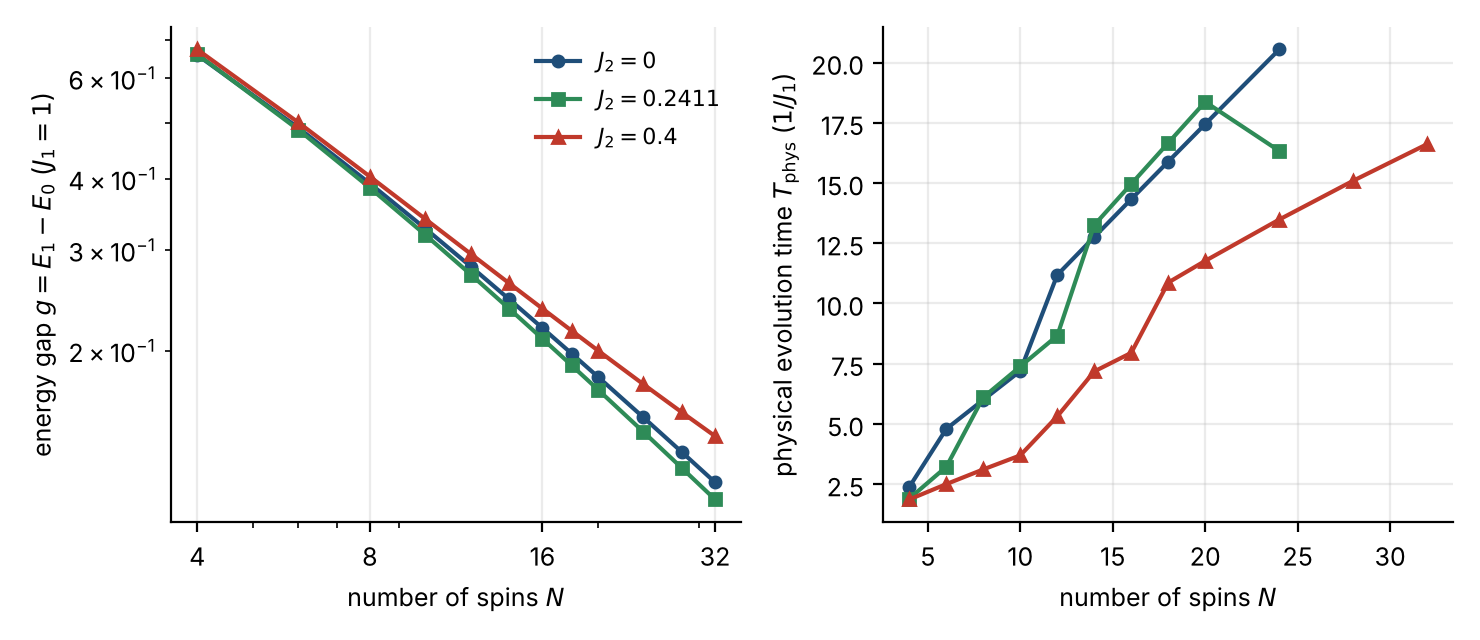
\includegraphics[width=0.95\linewidth]{figures_tex/gap_and_time.png}
\caption{(a) Energy gap $g=E_1-E_0$ against $N$. (b) Physical evolution time $T_{\rm phys}$ of the guaranteed design ($\varepsilon=10^{-2}$): it grows because the filter must resolve the shrinking gap ($T_{\rm phys}=x\pi/g$). The jumps reflect the discrete choice of $x=T\Delta/\pi\in[0.4,2.5]$ made by the design search, not the physics.}\label{fig:gap}
\end{figure}


\section{Accuracy of the DMRG inputs}\label{sec:dmrg}
The filter design depends on $E_0$, $E_1$ (through $\Delta$) and $\gamma$, all computed by DMRG. Settings: SVD cutoff $10^{-14}$, energy tolerance $10^{-12}$, inner eigensolver tolerance $10^{-10}$, bond dimension up to 256. The excited state is found by adding the rank-one penalty $\lambda|\psi_0\rangle\langle\psi_0|$ to each local two-site problem, which returns the lowest state of any symmetry orthogonal to the ground state without building the large projector operator. Table~\ref{tab:ed} compares with exact diagonalisation (ED, used for testing only; $N\leq20$); Table~\ref{tab:cons} compares two independent runs where no exact answer exists ($N=24$--$32$); Table~\ref{tab:gam} checks the MPS computation of $\gamma$ used above $N=14$. Fig.~\ref{fig:dmrg} summarises.
\begin{figure}[htbp]
\centering
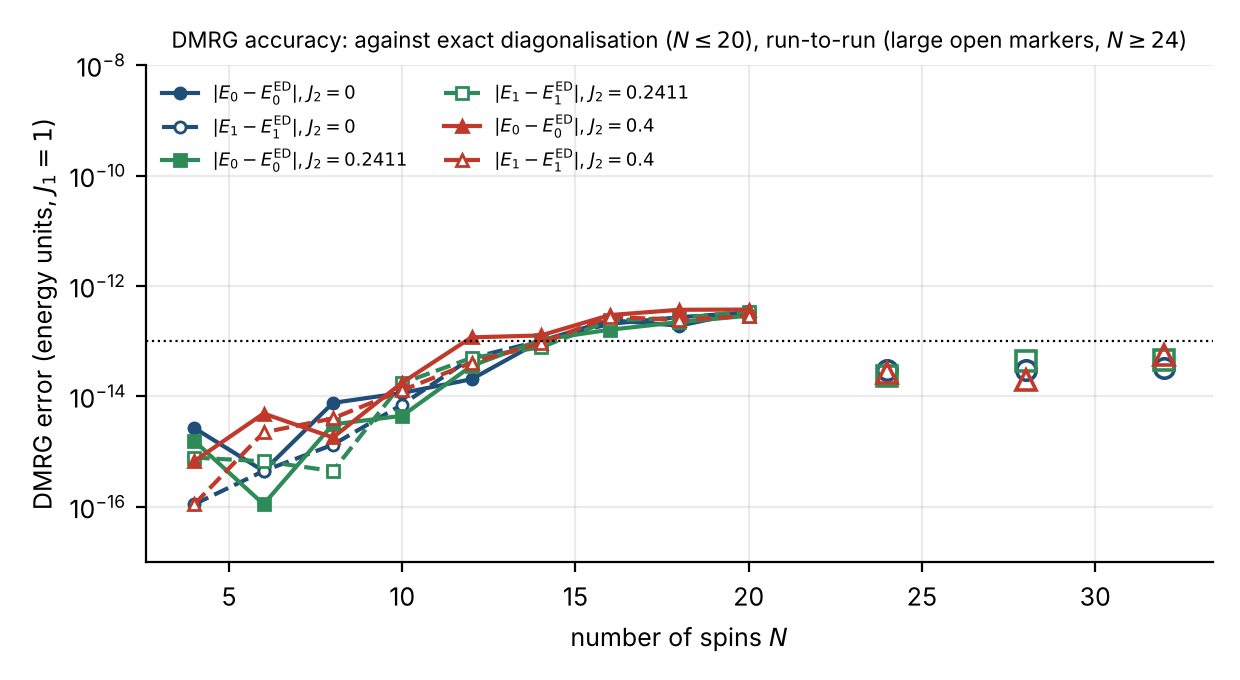
\includegraphics[width=0.95\linewidth]{figures_tex/dmrg_accuracy.png}
\caption{DMRG energy errors. Small markers: against exact diagonalisation. Large open markers ($N\geq24$): largest run-to-run difference of $E_0,E_1$. Dotted line: $10^{-13}$.}\label{fig:dmrg}
\end{figure}
{\small
\begin{longtable}{rrrrrrrr}
\caption{DMRG against exact diagonalisation (ED). All energies in units of $J_1$.}\label{tab:ed}\\
\toprule
$N$ & $J_2$ & $|E_0-E_0^{\rm ED}|$ & $|E_1-E_1^{\rm ED}|$ & $|E_{\rm top}-E_{\rm top}^{\rm ED}|$ & $1-|\langle\psi_0|\psi_0^{\rm ED}\rangle|^2$ & max bond & conv. \\
\midrule
\endfirsthead
\toprule
$N$ & $J_2$ & $|E_0-E_0^{\rm ED}|$ & $|E_1-E_1^{\rm ED}|$ & $|E_{\rm top}-E_{\rm top}^{\rm ED}|$ & $1-|\langle\psi_0|\psi_0^{\rm ED}\rangle|^2$ & max bond & conv. \\
\midrule
\endhead
\bottomrule
\endfoot
4 & 0 & $1.1\times10^{-15}$ & $8.9\times10^{-16}$ & $7.8\times10^{-16}$ & $4.4\times10^{-16}$ & 4 & yes \\
6 & 0 & $3.1\times10^{-15}$ & $1.3\times10^{-15}$ & $1.3\times10^{-15}$ & $1.3\times10^{-15}$ & 8 & yes \\
8 & 0 & $2.1\times10^{-15}$ & $1.3\times10^{-15}$ & $2.6\times10^{-15}$ & $1.3\times10^{-15}$ & 16 & yes \\
10 & 0 & $7.1\times10^{-15}$ & $6.7\times10^{-15}$ & $7.1\times10^{-15}$ & $1.3\times10^{-15}$ & 32 & yes \\
12 & 0 & $2.0\times10^{-14}$ & $5.4\times10^{-14}$ & $5.8\times10^{-15}$ & $4.4\times10^{-15}$ & 45 & yes \\
14 & 0 & $1.3\times10^{-13}$ & $1.6\times10^{-13}$ & $2.7\times10^{-15}$ & $3.2\times10^{-14}$ & 48 & yes \\
16 & 0 & $2.4\times10^{-13}$ & $2.1\times10^{-13}$ & $1.4\times10^{-14}$ & $4.4\times10^{-14}$ & 62 & yes \\
18 & 0 & $1.9\times10^{-13}$ & $2.7\times10^{-13}$ & $8.9\times10^{-16}$ & $6.0\times10^{-14}$ & 66 & yes \\
20 & 0 & $3.5\times10^{-13}$ & $3.3\times10^{-13}$ & $2.7\times10^{-14}$ & $8.1\times10^{-14}$ & 77 & yes \\
4 & 0.2411 & $1.6\times10^{-15}$ & $1.1\times10^{-16}$ & $3.4\times10^{-16}$ & $4.4\times10^{-16}$ & 4 & yes \\
6 & 0.2411 & $1.8\times10^{-15}$ & $8.9\times10^{-16}$ & $1.3\times10^{-15}$ & $2.2\times10^{-16}$ & 8 & yes \\
8 & 0.2411 & $4.7\times10^{-16}$ & $4.0\times10^{-15}$ & $9.6\times10^{-16}$ & $1.8\times10^{-15}$ & 16 & yes \\
10 & 0.2411 & $9.8\times10^{-15}$ & $3.7\times10^{-14}$ & $1.8\times10^{-15}$ & $4.4\times10^{-16}$ & 32 & yes \\
12 & 0.2411 & $2.1\times10^{-14}$ & $5.3\times10^{-14}$ & $8.9\times10^{-16}$ & $6.4\times10^{-15}$ & 43 & yes \\
14 & 0.2411 & $1.0\times10^{-13}$ & $9.6\times10^{-14}$ & $5.3\times10^{-15}$ & $2.9\times10^{-14}$ & 52 & yes \\
16 & 0.2411 & $1.6\times10^{-13}$ & $2.4\times10^{-13}$ & $6.2\times10^{-15}$ & $5.1\times10^{-14}$ & 65 & yes \\
18 & 0.2411 & $2.2\times10^{-13}$ & $2.6\times10^{-13}$ & $1.3\times10^{-13}$ & $5.4\times10^{-14}$ & 68 & yes \\
20 & 0.2411 & $2.9\times10^{-13}$ & $3.4\times10^{-13}$ & $3.6\times10^{-15}$ & $6.3\times10^{-14}$ & 77 & yes \\
4 & 0.4 & $9.0\times10^{-16}$ & $1.1\times10^{-16}$ & $8.1\times10^{-16}$ & $2.2\times10^{-16}$ & 4 & yes \\
6 & 0.4 & $8.4\times10^{-15}$ & $4.4\times10^{-16}$ & $1.8\times10^{-15}$ & $1.0\times10^{-17}$ & 8 & yes \\
8 & 0.4 & $4.0\times10^{-15}$ & $3.9\times10^{-14}$ & $8.0\times10^{-15}$ & $8.9\times10^{-16}$ & 16 & yes \\
10 & 0.4 & $4.7\times10^{-16}$ & $4.3\times10^{-14}$ & $1.2\times10^{-14}$ & $1.1\times10^{-15}$ & 29 & yes \\
12 & 0.4 & $1.1\times10^{-13}$ & $4.7\times10^{-14}$ & $1.3\times10^{-14}$ & $2.0\times10^{-14}$ & 46 & yes \\
14 & 0.4 & $1.0\times10^{-13}$ & $1.3\times10^{-13}$ & $8.0\times10^{-15}$ & $3.5\times10^{-14}$ & 59 & yes \\
16 & 0.4 & $3.0\times10^{-13}$ & $2.8\times10^{-13}$ & $8.0\times10^{-15}$ & $6.8\times10^{-14}$ & 70 & yes \\
18 & 0.4 & $3.7\times10^{-13}$ & $2.4\times10^{-13}$ & $8.9\times10^{-16}$ & $7.9\times10^{-14}$ & 79 & yes \\
20 & 0.4 & $3.7\times10^{-13}$ & $2.9\times10^{-13}$ & $5.3\times10^{-15}$ & $6.8\times10^{-14}$ & 86 & yes \\
\end{longtable}
}
{\small
\begin{longtable}{rrrrrrrrr}
\caption{No exact reference: two independent DMRG runs from different random starts. $\Delta E$ is the difference between the runs; the variance is $\langle H^2\rangle-\langle H\rangle^2$ of each state.}\label{tab:cons}\\
\toprule
$N$ & $J_2$ & $|\Delta E_0|$ & $|\Delta E_1|$ & $|\Delta E_{\rm top}|$ & $1-|\langle\psi_0|\psi_0'\rangle|^2$ & var.\ of $\psi_0$ & var.\ of $\psi_1$ & conv. \\
\midrule
\endfirsthead
\toprule
$N$ & $J_2$ & $|\Delta E_0|$ & $|\Delta E_1|$ & $|\Delta E_{\rm top}|$ & $1-|\langle\psi_0|\psi_0'\rangle|^2$ & var.\ of $\psi_0$ & var.\ of $\psi_1$ & conv. \\
\midrule
\endhead
\bottomrule
\endfoot
24 & 0 & $3.0\times10^{-14}$ & $3.6\times10^{-15}$ & $2.9\times10^{-14}$ & $4.7\times10^{-14}$ & $3.2\times10^{-12}$ & $2.4\times10^{-12}$ & yes \\
28 & 0 & $1.4\times10^{-14}$ & $3.0\times10^{-14}$ & $8.8\times10^{-14}$ & $1.8\times10^{-14}$ & $3.2\times10^{-12}$ & $2.9\times10^{-12}$ & yes \\
32 & 0 & $3.2\times10^{-14}$ & $1.6\times10^{-14}$ & $1.2\times10^{-13}$ & $2.4\times10^{-14}$ & $6.3\times10^{-12}$ & $3.4\times10^{-12}$ & yes \\
24 & 0.2411 & $7.1\times10^{-15}$ & $2.3\times10^{-14}$ & $1.5\times10^{-14}$ & $5.2\times10^{-14}$ & $2.4\times10^{-12}$ & $2.4\times10^{-12}$ & yes \\
28 & 0.2411 & $2.5\times10^{-14}$ & $4.4\times10^{-14}$ & $2.8\times10^{-14}$ & $3.5\times10^{-14}$ & $2.2\times10^{-12}$ & $3.3\times10^{-12}$ & yes \\
32 & 0.2411 & $4.6\times10^{-14}$ & $1.8\times10^{-14}$ & $7.3\times10^{-14}$ & $3.0\times10^{-14}$ & $5.2\times10^{-12}$ & $3.6\times10^{-12}$ & yes \\
24 & 0.4 & $2.0\times10^{-14}$ & $2.7\times10^{-14}$ & $3.6\times10^{-14}$ & $2.3\times10^{-14}$ & $3.0\times10^{-12}$ & $2.3\times10^{-12}$ & yes \\
28 & 0.4 & $2.0\times10^{-14}$ & $7.1\times10^{-15}$ & $6.2\times10^{-14}$ & $4.3\times10^{-14}$ & $4.0\times10^{-12}$ & $3.0\times10^{-12}$ & yes \\
32 & 0.4 & $5.7\times10^{-14}$ & $7.1\times10^{-15}$ & $9.2\times10^{-14}$ & $5.2\times10^{-14}$ & $5.5\times10^{-12}$ & $3.3\times10^{-12}$ & yes \\
\end{longtable}
}
{\small
\begin{longtable}{rrrrr}
\caption{The trial-state weight $\gamma$ computed by MPS contraction (used for $N>14$) against the dense overlap with the exact ground state (testing only).}\label{tab:gam}\\
\toprule
$N$ & $J_2$ & $\gamma$ (dense, exact GS) & $\gamma$ (MPS contraction) & difference \\
\midrule
\endfirsthead
\toprule
$N$ & $J_2$ & $\gamma$ (dense, exact GS) & $\gamma$ (MPS contraction) & difference \\
\midrule
\endhead
\bottomrule
\endfoot
16 & 0 & 0.60680231 & 0.60680231 & $1.5\times10^{-9}$ \\
18 & 0 & 0.55463710 & 0.55463710 & $2.5\times10^{-9}$ \\
16 & 0.2411 & 0.73678413 & 0.73678413 & $7.0\times10^{-10}$ \\
18 & 0.2411 & 0.69454313 & 0.69454313 & $2.7\times10^{-10}$ \\
16 & 0.4 & 0.91693867 & 0.91693867 & $7.8\times10^{-12}$ \\
18 & 0.4 & 0.90003595 & 0.90003595 & $2.8\times10^{-10}$ \\
\end{longtable}
}

Run-to-run agreement shows that the solves are converged and reproducible; it does not prove they sit at the true minimum. The weight $\gamma$ is the least accurate input (first order in the state error): it agrees with the exact overlap to $2.5e-09$.

\section{The certified bandwidth}\label{sec:bandwidth}
The scaling $H_s=(H-E_0)/W$ requires $W\geq E_{\rm top}-E_0$. DMRG on $-H$ is variational from the wrong side ($E_{\rm top}^{\rm DMRG}\leq E_{\rm top}$), so it cannot supply a safe $W$. Instead we use \textbf{Weyl's inequality}: the largest eigenvalue of a sum is at most the sum of the largest eigenvalues. A bond $J\,\mathbf S\!\cdot\!\mathbf S$ has eigenvalues $J/4$ (triplet) and $-3J/4$ (singlet), so for $J_1,J_2\geq0$
\[
E_{\rm top}\;\leq\;\tfrac{N-1}{4}J_1+\tfrac{N-2}{4}J_2,\qquad W=\tfrac{N-1}{4}J_1+\tfrac{N-2}{4}J_2-E_0 .
\]
The fully polarised state attains the bound, so $W=E_{\rm top}-E_0$ exactly (Table~\ref{tab:bw}). The Pauli-term bound used earlier ($\sum|c_\beta|-E_0$) is $1.6$--$1.9\times$ larger. \textbf{$W$ cancels in the cost:} $\alpha_{\rm scaled}=\alpha/W^2$ and $T=x\pi W/g$, so $n\propto\alpha T^2\propto\alpha/g^2$ and $T_{\rm phys}=x\pi/g$ do not depend on $W$; a looser $W$ only widens the suppression window. Switching from the earlier Pauli-$\ell_1$ bandwidth to the Weyl bandwidth changed the guaranteed step count by a factor 0.63--1.14 (median 0.99) and the physical time by 0.67--1.50, over 59 matching designs.
{\small
\begin{longtable}{rrrrrr}
\caption{The certified bandwidth $W=\sum_{\rm bonds}\lambda_{\max}-E_0$ against the DMRG value of $E_{\rm top}-E_0$ and against the looser Pauli bound used earlier.}\label{tab:bw}\\
\toprule
$N$ & $J_2$ & $W$ (Weyl) & $|W-(E_{\rm top}-E_0)_{\rm DMRG}|$ & $W$ (Pauli-$\ell_1$, earlier) & $\ell_1$ / Weyl \\
\midrule
\endfirsthead
\toprule
$N$ & $J_2$ & $W$ (Weyl) & $|W-(E_{\rm top}-E_0)_{\rm DMRG}|$ & $W$ (Pauli-$\ell_1$, earlier) & $\ell_1$ / Weyl \\
\midrule
\endhead
\bottomrule
\endfoot
4 & 0 & 2.36603 & $0$ & 3.8660 & 1.63 \\
8 & 0 & 5.12493 & $8.9\times10^{-16}$ & 8.6249 & 1.68 \\
12 & 0 & 7.89209 & $3.6\times10^{-15}$ & 13.3921 & 1.70 \\
16 & 0 & 10.66174 & $1.8\times10^{-15}$ & 18.1617 & 1.70 \\
20 & 0 & 13.43247 & $4.3\times10^{-14}$ & 22.9325 & 1.71 \\
24 & 0 & 16.20379 & $1.8\times10^{-14}$ & 27.7038 & 1.71 \\
28 & 0 & 18.97544 & $9.6\times10^{-14}$ & 32.4754 & 1.71 \\
32 & 0 & 21.74732 & $2.4\times10^{-13}$ & 37.2473 & 1.71 \\
4 & 0.2411 & 2.40929 & $0$ & 4.1504 & 1.72 \\
8 & 0.2411 & 5.24665 & $0$ & 9.4700 & 1.80 \\
12 & 0.2411 & 8.09083 & $0$ & 14.7963 & 1.83 \\
16 & 0.2411 & 10.93717 & $0$ & 20.1249 & 1.84 \\
20 & 0.2411 & 13.78446 & $2.8\times10^{-14}$ & 25.4544 & 1.85 \\
24 & 0.2411 & 16.63227 & $0$ & 30.7844 & 1.85 \\
28 & 0.2411 & 19.48038 & $8.5\times10^{-14}$ & 36.1147 & 1.85 \\
32 & 0.2411 & 22.32868 & $2.6\times10^{-13}$ & 41.4452 & 1.86 \\
4 & 0.4 & 2.45678 & $0$ & 4.3568 & 1.77 \\
8 & 0.4 & 5.37519 & $5.3\times10^{-15}$ & 10.0752 & 1.87 \\
12 & 0.4 & 8.29563 & $7.1\times10^{-15}$ & 15.7956 & 1.90 \\
16 & 0.4 & 11.21667 & $0$ & 21.5167 & 1.92 \\
20 & 0.4 & 14.13794 & $0$ & 27.2379 & 1.93 \\
24 & 0.4 & 17.05933 & $0$ & 32.9593 & 1.93 \\
28 & 0.4 & 19.98077 & $0$ & 38.6808 & 1.94 \\
32 & 0.4 & 22.90224 & $2.9\times10^{-13}$ & 44.4022 & 1.94 \\
\end{longtable}
}


\section{Small chains: guaranteed designs}\label{sec:small}
Table~\ref{tab:gd} gives the design (pulses, steps, times) and the proven and measured infidelity for $N\leq14$ at $\varepsilon=10^{-2}$; Table~\ref{tab:gc} the gate counts. The proven bound is below $\varepsilon$ by construction, and the measured infidelity is smaller by a factor of about 6--40 (Fig.~\ref{fig:bound}), because the Trotter part of the bound is a worst case over all states.
{\small
\begin{longtable}{rrrrrrrrrr}
\caption{Guaranteed designs for $\varepsilon=10^{-2}$, $N\leq14$. $m$ = pulses, $n$ = Trotter steps, $T=\sum t_i$ in units of $1/W$, $T_{\rm phys}=T/W$ in units of $1/J_1$, $\eta$ = certified suppression, $p_g$ = proven lower bound on the success probability, ``bound'' = proven upper bound on the infidelity $1-F$, ``measured'' = simulated against the exact ground state.}\label{tab:gd}\\
\toprule
$N$ & $J_2$ & $m$ & $n$ & $T$ & $T_{\rm phys}$ & $\eta$ & $p_g$ & bound on $1-F$ & measured $1-F$ \\
\midrule
\endfirsthead
\toprule
$N$ & $J_2$ & $m$ & $n$ & $T$ & $T_{\rm phys}$ & $\eta$ & $p_g$ & bound on $1-F$ & measured $1-F$ \\
\midrule
\endhead
\bottomrule
\endfoot
4 & 0 & 4 & 85 & 5.6 & 2.38 & 0.143 & 0.535 & $9.91\times10^{-3}$ & $2.87\times10^{-4}$ \\
6 & 0 & 4 & 590 & 17.9 & 4.79 & 0.092 & 0.718 & $9.99\times10^{-3}$ & $7.73\times10^{-4}$ \\
8 & 0 & 6 & 1\,817 & 30.8 & 6.00 & 0.100 & 0.632 & $10.00\times10^{-3}$ & $1.29\times10^{-3}$ \\
10 & 0 & 6 & 3\,917 & 46.8 & 7.20 & 0.081 & 0.500 & $10.00\times10^{-3}$ & $1.19\times10^{-3}$ \\
12 & 0 & 8 & 8\,797 & 88.3 & 11.18 & 0.050 & 0.600 & $9.99\times10^{-3}$ & $3.18\times10^{-4}$ \\
14 & 0 & 8 & 17\,822 & 118.4 & 12.76 & 0.062 & 0.595 & $9.47\times10^{-3}$ & $6.35\times10^{-4}$ \\
4 & 0.2411 & 4 & 94 & 4.6 & 1.90 & 0.313 & 0.631 & $9.93\times10^{-3}$ & $9.78\times10^{-4}$ \\
6 & 0.2411 & 4 & 578 & 12.3 & 3.22 & 0.190 & 0.594 & $10.00\times10^{-3}$ & $1.57\times10^{-3}$ \\
8 & 0.2411 & 6 & 2\,398 & 32.0 & 6.11 & 0.099 & 0.687 & $10.00\times10^{-3}$ & $2.42\times10^{-4}$ \\
10 & 0.2411 & 6 & 5\,777 & 49.2 & 7.38 & 0.113 & 0.691 & $10.00\times10^{-3}$ & $5.03\times10^{-4}$ \\
12 & 0.2411 & 6 & 10\,960 & 70.1 & 8.66 & 0.095 & 0.574 & $10.00\times10^{-3}$ & $4.09\times10^{-4}$ \\
14 & 0.2411 & 8 & 24\,027 & 126.1 & 13.25 & 0.059 & 0.694 & $9.36\times10^{-3}$ & $3.83\times10^{-4}$ \\
4 & 0.4 & 4 & 76 & 4.6 & 1.87 & 0.486 & 0.891 & $9.98\times10^{-3}$ & $1.64\times10^{-4}$ \\
6 & 0.4 & 4 & 394 & 9.8 & 2.50 & 0.399 & 0.739 & $9.98\times10^{-3}$ & $4.13\times10^{-4}$ \\
8 & 0.4 & 4 & 1\,059 & 16.7 & 3.11 & 0.286 & 0.579 & $9.98\times10^{-3}$ & $4.89\times10^{-4}$ \\
10 & 0.4 & 4 & 2\,890 & 25.3 & 3.69 & 0.321 & 0.613 & $10.00\times10^{-3}$ & $7.61\times10^{-4}$ \\
12 & 0.4 & 6 & 5\,318 & 44.1 & 5.31 & 0.189 & 0.562 & $10.00\times10^{-3}$ & $4.85\times10^{-4}$ \\
14 & 0.4 & 6 & 10\,575 & 70.0 & 7.18 & 0.164 & 0.689 & $10.00\times10^{-3}$ & $4.56\times10^{-4}$ \\
\end{longtable}
}
{\small
\begin{longtable}{rrrrrrrrrr}
\caption{Gate counts of the guaranteed designs ($\varepsilon=10^{-2}$, all-to-all connectivity). Totals include the trial circuit. ``RZZ / accept'' = RZZ total divided by the success probability: the expected RZZ per accepted run. Non-Clifford rotations = $R_z$ plus RZZ gates whose angle is not a multiple of $\pi/2$.}\label{tab:gc}\\
\toprule
$N$ & $J_2$ & RZZ trial & RZZ filter & RZZ total & RZZ filter (direct) & non-Cliff.\ rot. (level 3) & non-Cliff.\ rot. (direct) & depth & RZZ / accept \\
\midrule
\endfirsthead
\toprule
$N$ & $J_2$ & RZZ trial & RZZ filter & RZZ total & RZZ filter (direct) & non-Cliff.\ rot. (level 3) & non-Cliff.\ rot. (direct) & depth & RZZ / accept \\
\midrule
\endhead
\bottomrule
\endfoot
4 & 0 & 9 & 1\,530 & 1\,539 & 3\,060 & 1\,573 & 854 & 4\,458 & 2\,876 \\
6 & 0 & 15 & 17\,700 & 17\,715 & 35\,400 & 11\,867 & 9\,444 & 47\,850 & 24\,643 \\
8 & 0 & 21 & 76\,314 & 76\,335 & 152\,628 & 69\,139 & 39\,980 & 212\,671 & 120\,670 \\
10 & 0 & 27 & 211\,518 & 211\,545 & 423\,036 & 188\,133 & 109\,682 & 583\,737 & 422\,811 \\
12 & 0 & 33 & 580\,602 & 580\,635 & 1\,161\,204 & 510\,369 & 299\,106 & 1\,583\,586 & 967\,740 \\
14 & 0 & 38 & 1\,390\,116 & 1\,390\,154 & 2\,780\,232 & 1\,212\,062 & 712\,888 & 3\,778\,409 & 2\,335\,781 \\
4 & 0.2411 & 9 & 2\,820 & 2\,829 & 5\,640 & 2\,675 & 1\,508 & 7\,934 & 4\,474 \\
6 & 0.2411 & 15 & 31\,212 & 31\,227 & 62\,424 & 27\,811 & 16\,188 & 90\,228 & 52\,478 \\
8 & 0.2411 & 21 & 187\,044 & 187\,065 & 374\,088 & 163\,157 & 95\,926 & 551\,622 & 272\,308 \\
10 & 0.2411 & 27 & 589\,254 & 589\,281 & 1\,178\,508 & 508\,491 & 300\,410 & 1\,733\,204 & 852\,793 \\
12 & 0.2411 & 33 & 1\,380\,960 & 1\,380\,993 & 2\,761\,920 & 1\,183\,820 & 701\,446 & 4\,055\,326 & 2\,403\,340 \\
14 & 0.2411 & 39 & 3\,604\,050 & 3\,604\,089 & 7\,208\,100 & 3\,075\,621 & 1\,826\,060 & 10\,620\,082 & 5\,190\,564 \\
4 & 0.4 & 9 & 2\,280 & 2\,289 & 4\,560 & 2\,171 & 1\,220 & 7\,030 & 2\,567 \\
6 & 0.4 & 15 & 21\,276 & 21\,291 & 42\,552 & 18\,979 & 11\,036 & 58\,372 & 28\,786 \\
8 & 0.4 & 21 & 82\,602 & 82\,623 & 165\,204 & 72\,103 & 42\,364 & 237\,298 & 142\,638 \\
10 & 0.4 & 27 & 294\,780 & 294\,807 & 589\,560 & 254\,435 & 150\,284 & 797\,744 & 480\,264 \\
12 & 0.4 & 33 & 670\,068 & 670\,101 & 1\,340\,136 & 574\,485 & 340\,358 & 1\,914\,606 & 1\,191\,702 \\
14 & 0.4 & 39 & 1\,586\,250 & 1\,586\,289 & 3\,172\,500 & 1\,353\,765 & 803\,706 & 4\,399\,348 & 2\,302\,554 \\
\end{longtable}
}
\begin{figure}[htbp]
\centering
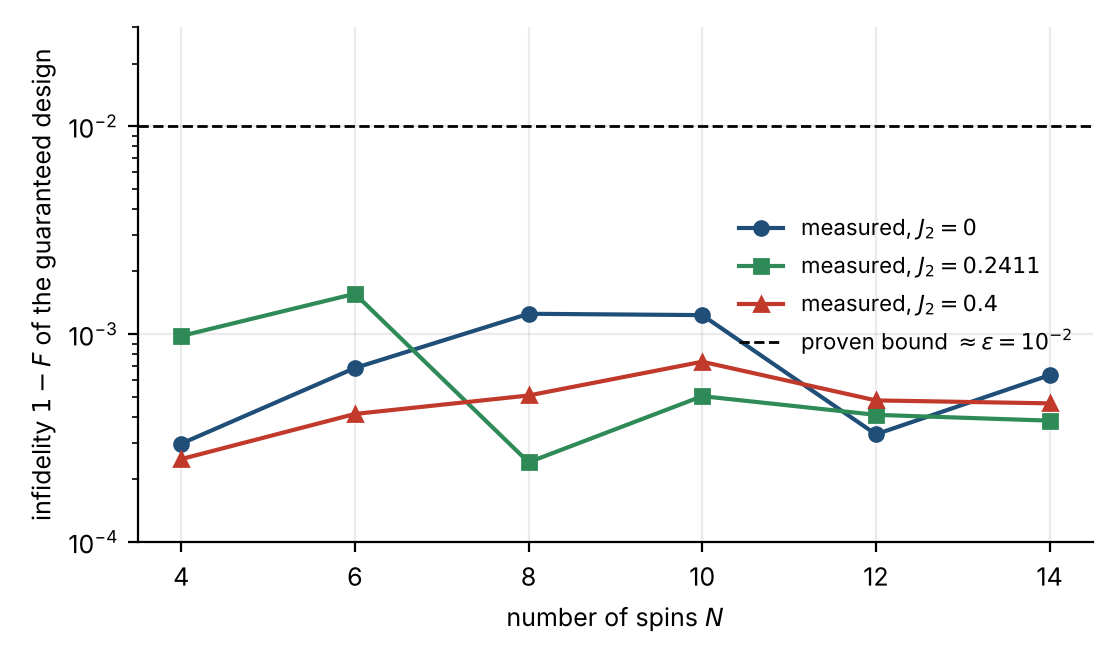
\includegraphics[width=0.55\linewidth]{figures_tex/bound_vs_measured.png}
\caption{Measured infidelity $1-F$ of the guaranteed designs ($N\leq14$, simulated against the exact ground state) compared with the proven bound (dashed), which equals the target $\varepsilon=10^{-2}$. The measured values lie well below the bound: it is never violated.}\label{fig:bound}
\end{figure}


\section{Guaranteed versus empirical designs}\label{sec:emp}
The empirical design is the smallest $n$ whose \emph{measured} infidelity meets $\varepsilon$; it needs the exact ground state and a simulation, so it shows what an ideal user could save. Table~\ref{tab:ge} and Fig.~\ref{fig:steps} compare. The proven design needs a large multiple of the empirical step count (and of the RZZ count, which is proportional to $n$) because its Trotter error bound is pessimistic.
{\small
\begin{longtable}{rrrrrrrr}
\caption{Guaranteed versus empirical (oracle) designs, $\varepsilon=10^{-2}$. The empirical design is the smallest $n$ whose \emph{measured} infidelity is below $\varepsilon$; it uses the exact ground state.}\label{tab:ge}\\
\toprule
$N$ & $J_2$ & $n$ guaranteed & $n$ empirical & ratio & RZZ guaranteed & RZZ empirical & measured $1-F$ (emp.) \\
\midrule
\endfirsthead
\toprule
$N$ & $J_2$ & $n$ guaranteed & $n$ empirical & ratio & RZZ guaranteed & RZZ empirical & measured $1-F$ (emp.) \\
\midrule
\endhead
\bottomrule
\endfoot
4 & 0 & 85 & 2 & 42$\times$ & 1\,539 & 45 & $6.83\times10^{-3}$ \\
6 & 0 & 590 & 5 & 118$\times$ & 17\,715 & 165 & $6.51\times10^{-3}$ \\
8 & 0 & 1\,817 & 11 & 165$\times$ & 76\,335 & 483 & $5.35\times10^{-3}$ \\
10 & 0 & 3\,917 & 10 & 392$\times$ & 211\,545 & 567 & $7.86\times10^{-3}$ \\
12 & 0 & 8\,797 & 29 & 303$\times$ & 580\,635 & 1\,947 & $5.75\times10^{-3}$ \\
14 & 0 & 17\,822 & 39 & 457$\times$ & 1\,390\,154 & 3\,080 & $3.45\times10^{-3}$ \\
4 & 0.2411 & 94 & 3 & 31$\times$ & 2\,829 & 99 & $5.78\times10^{-3}$ \\
6 & 0.2411 & 578 & 6 & 96$\times$ & 31\,227 & 339 & $9.52\times10^{-3}$ \\
8 & 0.2411 & 2\,398 & 11 & 218$\times$ & 187\,065 & 879 & $7.74\times10^{-3}$ \\
10 & 0.2411 & 5\,777 & 17 & 340$\times$ & 589\,281 & 1\,761 & $7.05\times10^{-3}$ \\
12 & 0.2411 & 10\,960 & 25 & 438$\times$ & 1\,380\,993 & 3\,183 & $7.80\times10^{-3}$ \\
14 & 0.2411 & 24\,027 & 41 & 586$\times$ & 3\,604\,089 & 6\,189 & $7.83\times10^{-3}$ \\
4 & 0.4 & 76 & 5 & 15$\times$ & 2\,289 & 159 & $3.54\times10^{-3}$ \\
6 & 0.4 & 394 & 6 & 66$\times$ & 21\,291 & 339 & $6.01\times10^{-3}$ \\
8 & 0.4 & 1\,059 & 11 & 96$\times$ & 82\,623 & 879 & $8.67\times10^{-3}$ \\
10 & 0.4 & 2\,890 & 16 & 181$\times$ & 294\,807 & 1\,659 & $9.47\times10^{-3}$ \\
12 & 0.4 & 5\,318 & 26 & 205$\times$ & 670\,101 & 3\,309 & $9.35\times10^{-3}$ \\
14 & 0.4 & 10\,575 & 38 & 278$\times$ & 1\,586\,289 & 5\,739 & $9.75\times10^{-3}$ \\
\end{longtable}
}
\begin{figure}[htbp]
\centering
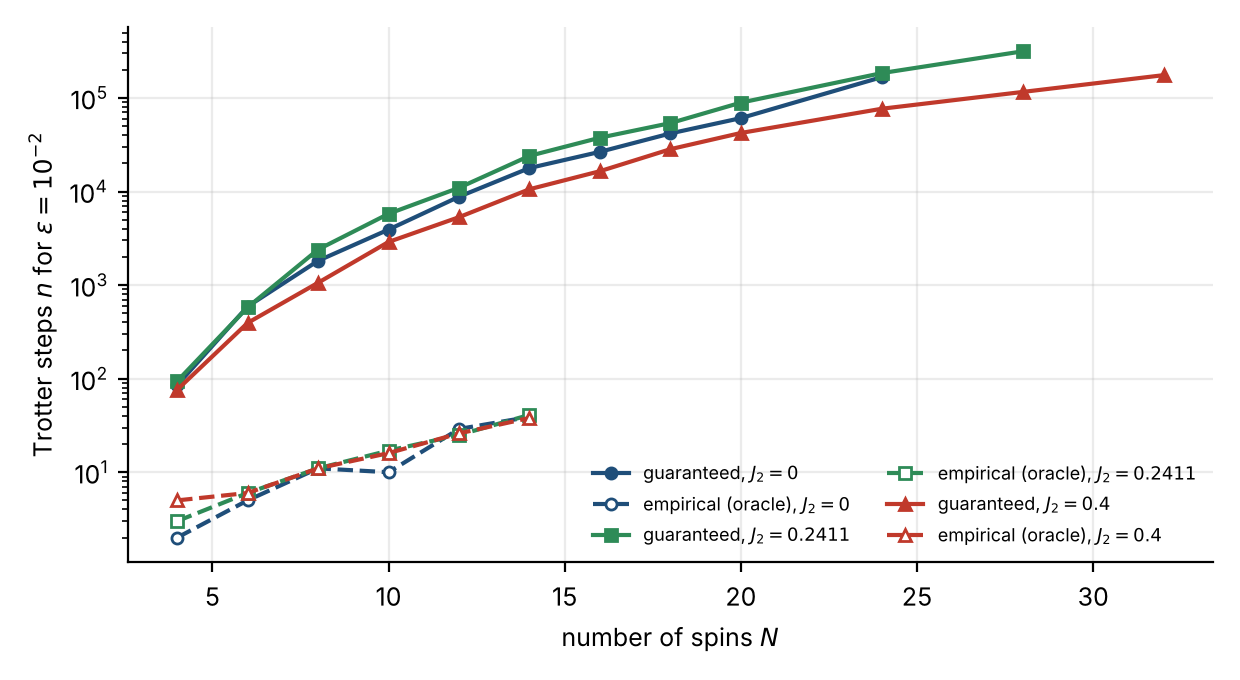
\includegraphics[width=0.95\linewidth]{figures_tex/steps_vs_N.png}
\caption{Trotter steps $n$ against $N$ for the guaranteed (solid) and empirical (dashed, $N\leq14$) designs, $\varepsilon=10^{-2}$.}\label{fig:steps}
\end{figure}


\section{Cost of one Trotter step}\label{sec:step}
All circuit costs are $n\times$ (cost of one step) plus the trial circuit. One step applies every term of $H$ once, controlled by the ancilla (Table~\ref{tab:ps}, Fig.~\ref{fig:step}). RZZ per step grows linearly in $N$ (one block per bond); $J_2\neq0$ roughly doubles it because the number of bonds doubles.
{\small
\begin{longtable}{rrrrrrrrr}
\caption{Transpiled cost of \emph{one} Trotter step of one pulse (every term of $H$, controlled by the ancilla). ``Line'': ancilla at the end of a linear chain of qubits (routing included; average of three transpiler seeds).}\label{tab:ps}\\
\toprule
$N$ & $J_2$ & Pauli terms & RZZ (level 3) & non-Cliff.\ rot. (level 3) & RZZ (direct) & non-Cliff.\ rot. (direct) & depth (level 3) & RZZ (line, level 3) \\
\midrule
\endfirsthead
\toprule
$N$ & $J_2$ & Pauli terms & RZZ (level 3) & non-Cliff.\ rot. (level 3) & RZZ (direct) & non-Cliff.\ rot. (direct) & depth (level 3) & RZZ (line, level 3) \\
\midrule
\endhead
\bottomrule
\endfoot
4 & 0 & 9 & 18 & 18 & 36 & 10 & 52 & 23 \\
8 & 0 & 21 & 42 & 38 & 84 & 22 & 117 & 59 \\
12 & 0 & 33 & 66 & 58 & 132 & 34 & 180 & 95 \\
16 & 0 & 45 & 90 & 78 & 180 & 46 & 244 & 131 \\
20 & 0 & 57 & 114 & 98 & 228 & 58 & 308 & 167 \\
24 & 0 & 69 & 138 & 118 & 276 & 70 & 372 & 208 \\
28 & 0 & 81 & 162 & 138 & 324 & 82 & 436 & 594 \\
32 & 0 & 93 & 186 & 158 & 372 & 94 & 500 & 710 \\
4 & 0.2411 & 15 & 30 & 28 & 60 & 16 & 84 & 49 \\
8 & 0.2411 & 39 & 78 & 68 & 156 & 40 & 230 & 148 \\
12 & 0.2411 & 63 & 126 & 108 & 252 & 64 & 370 & 258 \\
16 & 0.2411 & 87 & 174 & 148 & 348 & 88 & 497 & 362 \\
20 & 0.2411 & 111 & 222 & 188 & 444 & 112 & 650 & 466 \\
24 & 0.2411 & 135 & 270 & 228 & 540 & 136 & 746 & 1180 \\
28 & 0.2411 & 159 & 318 & 268 & 636 & 160 & 852 & 1942 \\
32 & 0.2411 & 183 & 366 & 308 & 732 & 184 & 1041 & 2472 \\
4 & 0.4 & 15 & 30 & 28 & 60 & 16 & 92 & 49 \\
8 & 0.4 & 39 & 78 & 68 & 156 & 40 & 224 & 148 \\
12 & 0.4 & 63 & 126 & 108 & 252 & 64 & 360 & 258 \\
16 & 0.4 & 87 & 174 & 148 & 348 & 88 & 497 & 362 \\
20 & 0.4 & 111 & 222 & 188 & 444 & 112 & 596 & 466 \\
24 & 0.4 & 135 & 270 & 228 & 540 & 136 & 724 & 1180 \\
28 & 0.4 & 159 & 318 & 268 & 636 & 160 & 904 & 1942 \\
32 & 0.4 & 183 & 366 & 308 & 732 & 184 & 1040 & 2472 \\
\end{longtable}
}
{\small
\begin{longtable}{rrrrrrrrrr}
\caption{Previous CX basis versus the RZZ basis, guaranteed designs at $\varepsilon=10^{-2}$. The direct compilation maps each CX onto one Clifford RZZ($\pi/2$) (ratio 1.00). At level 3 the CX circuit had already been re-synthesised to about 2.3 CX per ancilla-controlled Pauli rotation; in the RZZ basis each costs exactly two RZZ (one Clifford, one non-Clifford RZZ($\theta$)), about $0.86\times$ the level-3 CX count and half the direct count.}\label{tab:cxrzz}\\
\toprule
$N$ & $J_2$ & CX (level 3) & RZZ (level 3) & ratio & CX (direct) & RZZ (direct) & ratio & non-Cliff.\ $R_z$ (CX, level 3) & non-Cliff.\ rot. (RZZ, level 3) \\
\midrule
\endfirsthead
\toprule
$N$ & $J_2$ & CX (level 3) & RZZ (level 3) & ratio & CX (direct) & RZZ (direct) & ratio & non-Cliff.\ $R_z$ (CX, level 3) & non-Cliff.\ rot. (RZZ, level 3) \\
\midrule
\endhead
\bottomrule
\endfoot
6 & 0 & 20\,665 & 17\,715 & 0.86 & 35\,400 & 35\,400 & 1.00 & 27\,830 & 11\,867 \\
10 & 0 & 246\,798 & 211\,545 & 0.86 & 423\,036 & 423\,036 & 1.00 & 325\,289 & 188\,133 \\
14 & 0 & 1\,621\,841 & 1\,390\,154 & 0.86 & 2\,780\,232 & 2\,780\,232 & 1.00 & 2\,121\,074 & 1\,212\,062 \\
16 & 0 & 2\,787\,585 & 2\,389\,365 & 0.86 & 4\,778\,640 & 4\,778\,640 & 1.00 & 3\,637\,372 & 2\,070\,935 \\
20 & 0 & 8\,094\,836 & 6\,938\,439 & 0.86 & 13\,876\,764 & 13\,876\,764 & 1.00 & 10\,529\,667 & 5\,964\,812 \\
24 & 0 & 26\,862\,597 & 23\,025\,093 & 0.86 & 46\,050\,048 & 46\,050\,048 & 1.00 & 34\,871\,674 & 19\,688\,350 \\
6 & 0.2411 & 36\,429 & 31\,227 & 0.86 & 62\,424 & 62\,424 & 1.00 & 48\,075 & 27\,811 \\
10 & 0.2411 & 687\,490 & 589\,281 & 0.86 & 1\,178\,508 & 1\,178\,508 & 1.00 & 895\,612 & 508\,491 \\
14 & 0.2411 & 4\,204\,764 & 3\,604\,089 & 0.86 & 7\,208\,100 & 7\,208\,100 & 1.00 & 5\,454\,381 & 3\,075\,621 \\
16 & 0.2411 & 7\,630\,815 & 6\,540\,705 & 0.86 & 13\,081\,320 & 13\,081\,320 & 1.00 & 9\,886\,463 & 5\,563\,510 \\
20 & 0.2411 & 23\,065\,820 & 19\,770\,711 & 0.86 & 39\,541\,308 & 39\,541\,308 & 1.00 & 29\,834\,460 & 16\,742\,948 \\
24 & 0.2411 & 58\,045\,749 & 49\,753\,509 & 0.86 & 99\,506\,880 & 99\,506\,880 & 1.00 & 74\,999\,145 & 42\,014\,295 \\
6 & 0.4 & 24\,837 & 21\,291 & 0.86 & 42\,552 & 42\,552 & 1.00 & 32\,803 & 18\,979 \\
10 & 0.4 & 343\,937 & 294\,807 & 0.86 & 589\,560 & 589\,560 & 1.00 & 448\,127 & 254\,435 \\
14 & 0.4 & 1\,850\,664 & 1\,586\,289 & 0.86 & 3\,172\,500 & 3\,172\,500 & 1.00 & 2\,400\,780 & 1\,353\,765 \\
16 & 0.4 & 3\,346\,500 & 2\,868\,435 & 0.86 & 5\,736\,780 & 5\,736\,780 & 1.00 & 4\,335\,848 & 2\,439\,968 \\
20 & 0.4 & 10\,933\,742 & 9\,371\,787 & 0.86 & 18\,743\,460 & 18\,743\,460 & 1.00 & 14\,142\,388 & 7\,936\,651 \\
24 & 0.4 & 24\,147\,339 & 20\,697\,729 & 0.86 & 41\,395\,320 & 41\,395\,320 & 1.00 & 31\,200\,250 & 17\,478\,306 \\
32 & 0.4 & 74\,800\,245 & 64\,114\,509 & 0.86 & 128\,228\,832 & 128\,228\,832 & 1.00 & 96\,522\,564 & 53\,954\,580 \\
\end{longtable}
}
\begin{figure}[htbp]
\centering
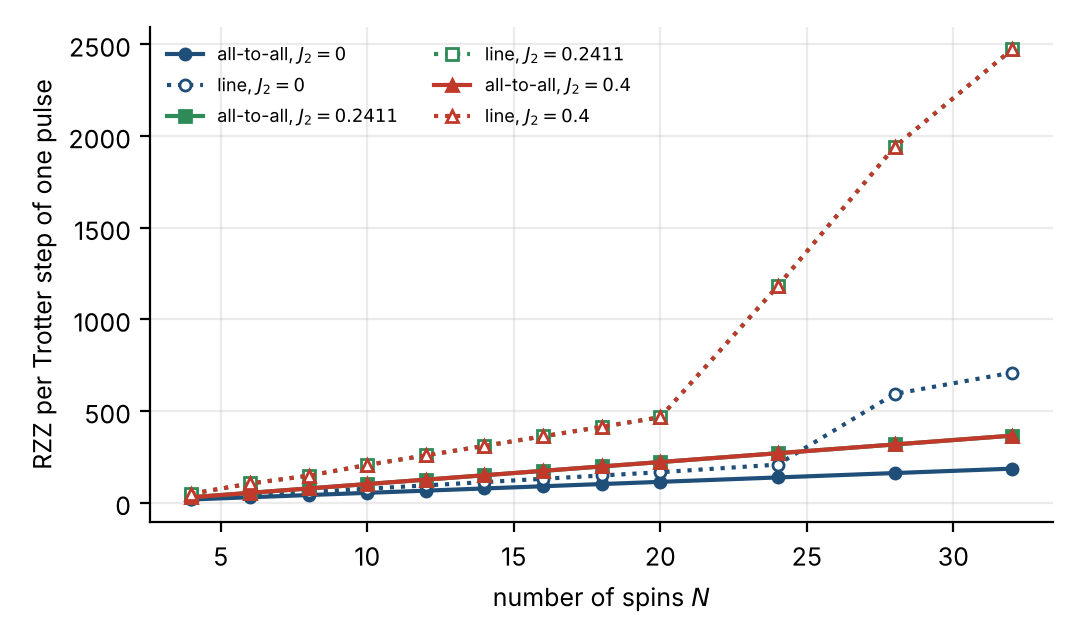
\includegraphics[width=0.7\linewidth]{figures_tex/rzz_per_step.png}
\caption{RZZ per Trotter step against $N$, all-to-all connectivity (solid) and line connectivity (dotted).}\label{fig:step}
\end{figure}


\section{Larger chains, $N$ up to 32}\label{sec:large}
Above $N=14$ nothing is simulated as a state vector: DMRG gives the energies and MPS, the trial circuit is simulated as an MPS to obtain $\gamma$, the filter is designed from $(\gamma,\Delta,\alpha)$, and circuits are counted. Tables~\ref{tab:large} and~\ref{tab:large1} give the guaranteed designs at $\varepsilon=10^{-2}$ and $10^{-1}$; Fig.~\ref{fig:cost} shows how the total RZZ and non-Clifford rotation counts grow (fits: $N^{5.1}$ ($J_2=0$, $N=6$--$24$), $N^{5.2}$ ($J_2=0.2411$, $N=6$--$28$), $N^{4.9}$ ($J_2=0.4$, $N=6$--$32$)). For $N=28,32$ at $J_2=0$ and $0.2411$ the trial circuit has $\gamma=0.31$--$0.51$ and the required suppression ($\eta_{\rm target}\approx0.07$--$0.10$) cannot be certified with at most 8 pulses; the looser target $\varepsilon=10^{-1}$ is feasible. This is a limit of the one-layer trial circuit, not of the filter.
{\small
\begin{longtable}{rrrrrrrrrrr}
\caption{Guaranteed designs for $N\geq14$, $\varepsilon=10^{-2}$ (DMRG/MPS only; circuits counted, not simulated). ``Not achievable'': no filter with at most 8 pulses meets the target for this trial state (Fig.~\ref{fig:gamma}). $^\ddagger$: fallback design.}\label{tab:large}\\
\toprule
$N$ & $J_2$ & $\gamma$ & $\Delta$ & $m$ & $n$ & $T_{\rm phys}$ & RZZ total (level 3) & RZZ (direct) & non-Cliff.\ rot. (direct) & $p_g$ \\
\midrule
\endfirsthead
\toprule
$N$ & $J_2$ & $\gamma$ & $\Delta$ & $m$ & $n$ & $T_{\rm phys}$ & RZZ total (level 3) & RZZ (direct) & non-Cliff.\ rot. (direct) & $p_g$ \\
\midrule
\endhead
\bottomrule
\endfoot
14 & 0 & 0.661 & 0.0265 & 8 & 17\,822 & 12.8 & $1.39\times10^{6}$ & $2.78\times10^{6}$ & $7.13\times10^{5}$ & 0.595 \\
16 & 0 & 0.606 & 0.0206 & 8 & 26\,548 & 14.3 & $2.39\times10^{6}$ & $4.78\times10^{6}$ & $1.22\times10^{6}$ & 0.527 \\
18 & 0 & 0.557 & 0.0164 & 8 & 41\,741 & 15.9 & $4.26\times10^{6}$ & $8.52\times10^{6}$ & $2.17\times10^{6}$ & 0.464 \\
20 & 0 & 0.514 & 0.0134 & 8 & 60\,863 & 17.4 & $6.94\times10^{6}$ & $1.39\times10^{7}$ & $3.53\times10^{6}$ & 0.402 \\
24 & 0 & 0.432 & 0.0094 & 8 & 166\,848 & 20.5 & $2.30\times10^{7}$ & $4.61\times10^{7}$ & $1.17\times10^{7}$ & 0.337 \\
28 & 0 & 0.365 & 0.0070 & -- & not achievable & -- & -- & -- & -- & -- \\
32 & 0 & 0.308 & 0.0054 & -- & not achievable & -- & -- & -- & -- & -- \\
14 & 0.2411 & 0.781 & 0.0249 & 8 & 24\,027 & 13.3 & $3.60\times10^{6}$ & $7.21\times10^{6}$ & $1.83\times10^{6}$ & 0.694 \\
16 & 0.2411 & 0.737 & 0.0192 & 8 & 37\,590 & 15.0 & $6.54\times10^{6}$ & $1.31\times10^{7}$ & $3.31\times10^{6}$ & 0.629 \\
18 & 0.2411 & 0.694 & 0.0153 & 8 & 53\,835 & 16.7 & $1.07\times10^{7}$ & $2.13\times10^{7}$ & $5.38\times10^{6}$ & 0.562 \\
20 & 0.2411 & 0.653 & 0.0124 & 8 & 89\,057 & 18.4 & $1.98\times10^{7}$ & $3.95\times10^{7}$ & $9.97\times10^{6}$ & 0.583 \\
24 & 0.2411 & 0.576 & 0.0087 & 8 & 184\,272 & 16.3 & $4.98\times10^{7}$ & $9.95\times10^{7}$ & $2.51\times10^{7}$ & 0.310 \\
28 & 0.2411 & 0.505 & 0.0064 & 8 & 314\,923 & 18.9 & $1.00\times10^{8}$ & $2.00\times10^{8}$ & $5.04\times10^{7}$ & 0.241 \\
32 & 0.2411 & 0.442 & 0.0049 & -- & not achievable & -- & -- & -- & -- & -- \\
14 & 0.4 & 0.933 & 0.0269 & 6 & 10\,575 & 7.2 & $1.59\times10^{6}$ & $3.17\times10^{6}$ & $8.04\times10^{5}$ & 0.689 \\
16 & 0.4 & 0.917 & 0.0211 & 6 & 16\,485 & 7.9 & $2.87\times10^{6}$ & $5.74\times10^{6}$ & $1.45\times10^{6}$ & 0.585 \\
18 & 0.4 & 0.900 & 0.0171 & 8 & 28\,336 & 10.9 & $5.61\times10^{6}$ & $1.12\times10^{7}$ & $2.83\times10^{6}$ & 0.602 \\
20 & 0.4 & 0.883 & 0.0142 & 8 & 42\,215 & 11.8 & $9.37\times10^{6}$ & $1.87\times10^{7}$ & $4.73\times10^{6}$ & 0.717 \\
24 & 0.4 & 0.849 & 0.0102 & 8 & 76\,658 & 13.5 & $2.07\times10^{7}$ & $4.14\times10^{7}$ & $1.04\times10^{7}$ & 0.621 \\
28 & 0.4 & 0.815 & 0.0078 & 8 & 115\,904 & 15.1 & $3.69\times10^{7}$ & $7.37\times10^{7}$ & $1.85\times10^{7}$ & 0.544 \\
32 & 0.4 & 0.782 & 0.0062 & 8 & 175\,176 & 16.6 & $6.41\times10^{7}$ & $1.28\times10^{8}$ & $3.22\times10^{7}$ & 0.470 \\
\end{longtable}
}
{\small
\begin{longtable}{rrrrrrrrr}
\caption{Guaranteed designs for $N\geq14$ at the looser target $\varepsilon=10^{-1}$.}\label{tab:large1}\\
\toprule
$N$ & $J_2$ & $m$ & $n$ & $T_{\rm phys}$ & RZZ total (level 3) & RZZ (direct) & non-Cliff.\ rot. (direct) & $p_g$ \\
\midrule
\endfirsthead
\toprule
$N$ & $J_2$ & $m$ & $n$ & $T_{\rm phys}$ & RZZ total (level 3) & RZZ (direct) & non-Cliff.\ rot. (direct) & $p_g$ \\
\midrule
\endhead
\bottomrule
\endfoot
16 & 0 & 6 & 3\,207 & 8.6 & $2.89\times10^{5}$ & $5.77\times10^{5}$ & $1.48\times10^{5}$ & 0.466 \\
18 & 0 & 6 & 4\,924 & 9.5 & $5.02\times10^{5}$ & $1.00\times10^{6}$ & $2.56\times10^{5}$ & 0.391 \\
20 & 0 & 6 & 7\,478 & 8.7 & $8.53\times10^{5}$ & $1.70\times10^{6}$ & $4.34\times10^{5}$ & 0.330 \\
24 & 0 & 8 & 18\,706 & 15.4 & $2.58\times10^{6}$ & $5.16\times10^{6}$ & $1.31\times10^{6}$ & 0.353 \\
28 & 0 & 8 & 34\,852 & 17.7 & $5.65\times10^{6}$ & $1.13\times10^{7}$ & $2.86\times10^{6}$ & 0.271 \\
32 & 0 & 8 & 75\,502 & 20.0 & $1.40\times10^{7}$ & $2.81\times10^{7}$ & $7.10\times10^{6}$ & 0.263 \\
16 & 0.2411 & 6 & 3\,768 & 6.0 & $6.56\times10^{5}$ & $1.31\times10^{6}$ & $3.32\times10^{5}$ & 0.479 \\
18 & 0.2411 & 6 & 5\,806 & 8.3 & $1.15\times10^{6}$ & $2.30\times10^{6}$ & $5.81\times10^{5}$ & 0.455 \\
20 & 0.2411 & 6 & 8\,597 & 9.2 & $1.91\times10^{6}$ & $3.82\times10^{6}$ & $9.63\times10^{5}$ & 0.390 \\
24 & 0.2411 & 8 & 20\,721 & 13.1 & $5.59\times10^{6}$ & $1.12\times10^{7}$ & $2.82\times10^{6}$ & 0.413 \\
28 & 0.2411 & 8 & 38\,728 & 12.6 & $1.23\times10^{7}$ & $2.46\times10^{7}$ & $6.20\times10^{6}$ & 0.315 \\
32 & 0.2411 & 8 & 82\,601 & 21.4 & $3.02\times10^{7}$ & $6.05\times10^{7}$ & $1.52\times10^{7}$ & 0.360 \\
16 & 0.4 & 4 & 2\,135 & 5.3 & $3.72\times10^{5}$ & $7.43\times10^{5}$ & $1.88\times10^{5}$ & 0.759 \\
18 & 0.4 & 6 & 2\,925 & 5.8 & $5.79\times10^{5}$ & $1.16\times10^{6}$ & $2.93\times10^{5}$ & 0.688 \\
20 & 0.4 & 6 & 4\,030 & 6.3 & $8.95\times10^{5}$ & $1.79\times10^{6}$ & $4.51\times10^{5}$ & 0.633 \\
24 & 0.4 & 6 & 6\,964 & 7.2 & $1.88\times10^{6}$ & $3.76\times10^{6}$ & $9.47\times10^{5}$ & 0.550 \\
28 & 0.4 & 6 & 11\,076 & 8.0 & $3.52\times10^{6}$ & $7.04\times10^{6}$ & $1.77\times10^{6}$ & 0.484 \\
32 & 0.4 & 6 & 21\,419 & 8.9 & $7.84\times10^{6}$ & $1.57\times10^{7}$ & $3.94\times10^{6}$ & 0.555 \\
\end{longtable}
}
\begin{figure}[htbp]
\centering
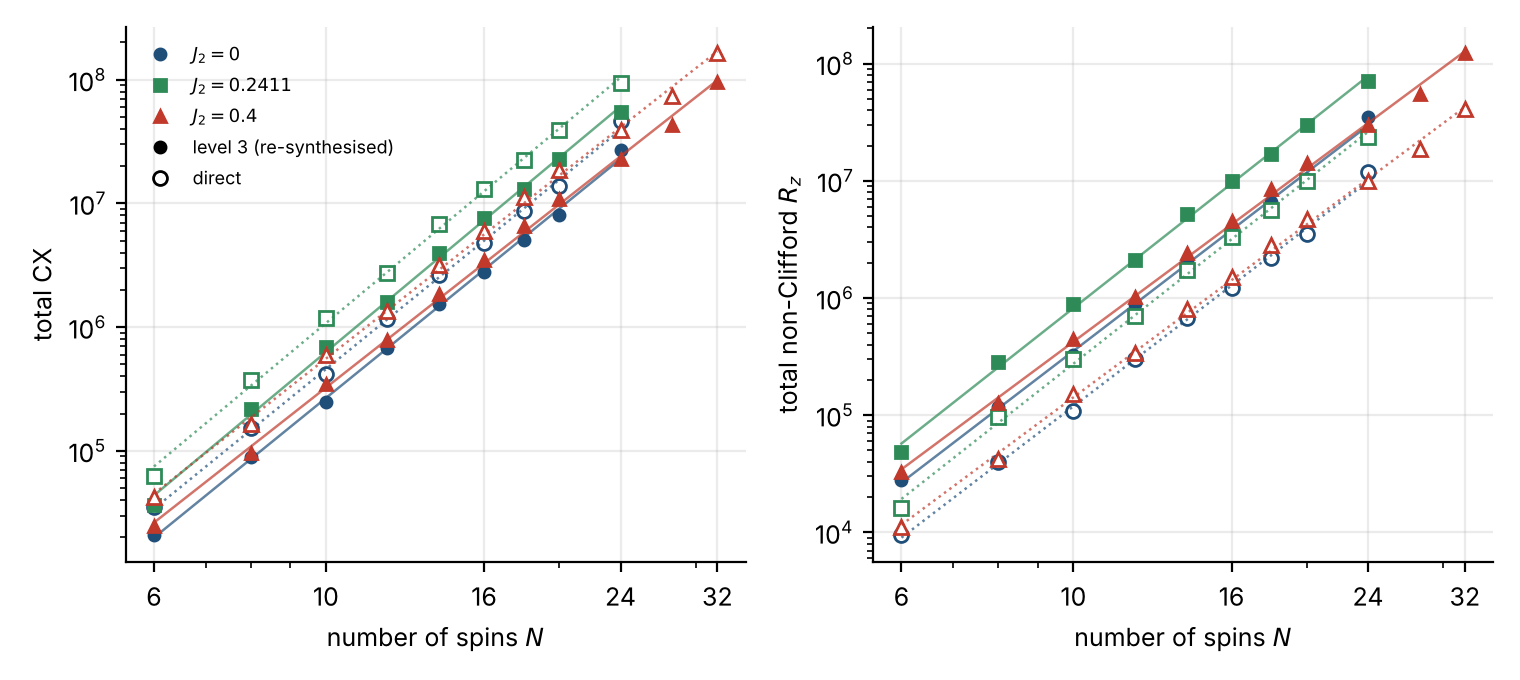
\includegraphics[width=0.95\linewidth]{figures_tex/cost_vs_N.png}
\caption{(a) Total RZZ and (b) total non-Clifford rotations of the guaranteed designs ($\varepsilon=10^{-2}$), log--log, with power-law fits (lines).}\label{fig:cost}
\end{figure}


\section{Dependence on the target $\varepsilon$}\label{sec:eps}
Tightening $\varepsilon$ needs both a stronger filter (smaller $\eta$) and fewer Trotter errors (more steps). Table~\ref{tab:eps} and Fig.~\ref{fig:eps} show three small cases.
{\small
\begin{longtable}{rrrlrrrrr}
\caption{Dependence on the target $\varepsilon$ for three small cases.}\label{tab:eps}\\
\toprule
$N$ & $J_2$ & $\varepsilon$ & design & $n$ & $m$ & $T_{\rm phys}$ & RZZ total & measured $1-F$ \\
\midrule
\endfirsthead
\toprule
$N$ & $J_2$ & $\varepsilon$ & design & $n$ & $m$ & $T_{\rm phys}$ & RZZ total & measured $1-F$ \\
\midrule
\endhead
\bottomrule
\endfoot
6 & 0 & 0.1 & guaranteed & 67 & 4 & 2.56 & $2.02\times10^{3}$ & $7.93\times10^{-3}$ \\
6 & 0 & 0.1 & empirical & 2 & 2 & 2.56 & $7.50\times10^{1}$ & $4.11\times10^{-2}$ \\
6 & 0 & 0.03 & guaranteed & 224 & 4 & 3.83 & $6.74\times10^{3}$ & $5.78\times10^{-4}$ \\
6 & 0 & 0.03 & empirical & 3 & 2 & 3.83 & $1.05\times10^{2}$ & $2.59\times10^{-2}$ \\
6 & 0 & 0.01 & guaranteed & 590 & 4 & 4.79 & $1.77\times10^{4}$ & $7.73\times10^{-4}$ \\
6 & 0 & 0.01 & empirical & 5 & 4 & 4.79 & $1.65\times10^{2}$ & $6.51\times10^{-3}$ \\
6 & 0 & 0.003 & guaranteed & 1\,807 & 6 & 6.39 & $5.42\times10^{4}$ & $1.02\times10^{-4}$ \\
6 & 0 & 0.003 & empirical & 9 & 5 & 6.39 & $2.85\times10^{2}$ & $3.17\times10^{-4}$ \\
6 & 0 & 0.001 & guaranteed & 4\,328 & 6 & 7.99 & $1.30\times10^{5}$ & $2.76\times10^{-5}$ \\
6 & 0 & 0.001 & empirical & 16 & 6 & 7.99 & $4.95\times10^{2}$ & $6.01\times10^{-4}$ \\
8 & 0 & 0.1 & guaranteed & 179 & 4 & 3.20 & $7.54\times10^{3}$ & $1.25\times10^{-2}$ \\
8 & 0 & 0.1 & empirical & 3 & 2 & 3.20 & $1.47\times10^{2}$ & $2.79\times10^{-2}$ \\
8 & 0 & 0.03 & guaranteed & 536 & 4 & 4.00 & $2.25\times10^{4}$ & $1.50\times10^{-3}$ \\
8 & 0 & 0.03 & empirical & 6 & 3 & 4.00 & $2.73\times10^{2}$ & $4.99\times10^{-3}$ \\
8 & 0 & 0.01 & guaranteed & 1\,817 & 6 & 6.00 & $7.63\times10^{4}$ & $1.29\times10^{-3}$ \\
8 & 0 & 0.01 & empirical & 11 & 4 & 6.00 & $4.83\times10^{2}$ & $5.35\times10^{-3}$ \\
8 & 0 & 0.003 & guaranteed & 5\,038 & 6 & 8.00 & $2.12\times10^{5}$ & $9.61\times10^{-5}$ \\
8 & 0 & 0.003 & empirical & 14 & 6 & 8.00 & $6.09\times10^{2}$ & $2.91\times10^{-3}$ \\
8 & 0 & 0.001 & guaranteed & 12\,061 & 8 & 10.00 & $5.07\times10^{5}$ & $5.88\times10^{-5}$ \\
8 & 0 & 0.001 & empirical & 24 & 7 & 10.00 & $1.03\times10^{3}$ & $9.21\times10^{-4}$ \\
6 & 0.4 & 0.1 & guaranteed & 79 & 4 & 2.50 & $4.28\times10^{3}$ & $1.19\times10^{-3}$ \\
6 & 0.4 & 0.1 & empirical & 3 & 2 & 2.50 & $1.77\times10^{2}$ & $5.15\times10^{-2}$ \\
6 & 0.4 & 0.03 & guaranteed & 197 & 4 & 2.50 & $1.07\times10^{4}$ & $1.75\times10^{-3}$ \\
6 & 0.4 & 0.03 & empirical & 4 & 2 & 2.50 & $2.31\times10^{2}$ & $2.75\times10^{-2}$ \\
6 & 0.4 & 0.01 & guaranteed & 394 & 4 & 2.50 & $2.13\times10^{4}$ & $4.13\times10^{-4}$ \\
6 & 0.4 & 0.01 & empirical & 6 & 3 & 2.50 & $3.39\times10^{2}$ & $6.01\times10^{-3}$ \\
6 & 0.4 & 0.003 & guaranteed & 1\,322 & 4 & 3.75 & $7.14\times10^{4}$ & $1.99\times10^{-4}$ \\
6 & 0.4 & 0.003 & empirical & 15 & 4 & 3.75 & $8.25\times10^{2}$ & $2.76\times10^{-3}$ \\
6 & 0.4 & 0.001 & guaranteed & 3\,033 & 4 & 3.75 & $1.64\times10^{5}$ & $1.39\times10^{-4}$ \\
6 & 0.4 & 0.001 & empirical & 26 & 4 & 3.75 & $1.42\times10^{3}$ & $9.63\times10^{-4}$ \\
\end{longtable}
}
\begin{figure}[htbp]
\centering
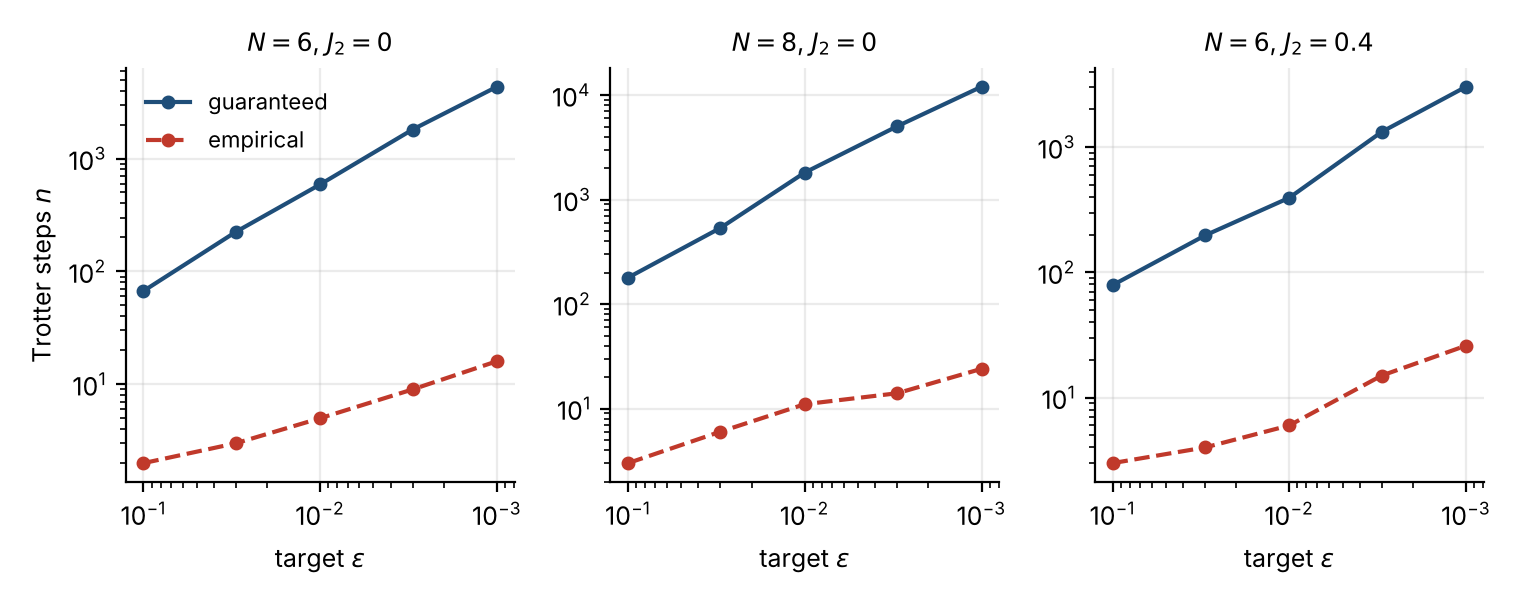
\includegraphics[width=0.95\linewidth]{figures_tex/eps_scan.png}
\caption{Trotter steps against target $\varepsilon$ for guaranteed (solid) and empirical (dashed) designs.}\label{fig:eps}
\end{figure}


\section{Checks and classical compute cost}\label{sec:checks}
\textbf{Gate-count method.} The per-step transpile times $n$ was compared with a full transpile of the real circuit in the RZZ basis at $n=48$ (4 pulses of 12 steps, all-to-all) for 66 cases: the RZZ count differed by at most 0 (level 3) and 0 (direct), the direct non-Clifford count by at most 0, and the level-3 non-Clifford estimate differed from the full transpile by -20\% to +19\% (it is not conservative: re-synthesis in the full circuit differs from the single-step transpile, so level-3 non-Clifford counts are $\pm20\%$ estimates, whereas the direct counts are exact); the level-3 depth estimate differed by -15\% to +7\%. \textbf{Bound violations:} 0 among the simulated designs. \textbf{Classical cost:} Table~\ref{tab:time}.
{\small
\begin{longtable}{rrrrrr}
\caption{Classical compute time per point (single core). The context build includes the three DMRG runs, the trial circuit and its overlap, $\alpha$ and the per-step transpile.}\label{tab:time}\\
\toprule
$N$ & points & context build (median s) & filter design (median s) & total per point (median s) & total per point (max s) \\
\midrule
\endfirsthead
\toprule
$N$ & points & context build (median s) & filter design (median s) & total per point (median s) & total per point (max s) \\
\midrule
\endhead
\bottomrule
\endfoot
4 & 3 & 0 & 22 & 25 & 31 \\
6 & 11 & 0 & 46 & 50 & 101 \\
8 & 7 & 0 & 78 & 85 & 111 \\
10 & 3 & 6 & 94 & 114 & 126 \\
12 & 3 & 349 & 119 & 497 & 526 \\
14 & 3 & 9 & 124 & 471 & 855 \\
16 & 6 & 11 & 108 & 120 & 126 \\
18 & 6 & 13 & 117 & 130 & 160 \\
20 & 6 & 22 & 112 & 129 & 166 \\
24 & 6 & 40 & 116 & 154 & 202 \\
28 & 6 & 51 & 116 & 153 & 235 \\
32 & 6 & 93 & 106 & 150 & 315 \\
\end{longtable}
}

\textbf{Points without a certified design:}
\begin{itemize}
\item $N=28$, $J_2=0$, $\varepsilon=0.01$: $\gamma=0.365$
\item $N=32$, $J_2=0$, $\varepsilon=0.01$: $\gamma=0.308$
\item $N=32$, $J_2=0.2411$, $\varepsilon=0.01$: $\gamma=0.442$
\end{itemize}



\section{First- versus second-order Trotter formula}\label{sec:second}
The same filter designs (pulse times and phases of the guaranteed designs) with the second-order (Strang) formula and its commutator bound (Childs, Su, Tran, Wiebe and Zhu, arXiv:1912.08854, Proposition~16, Eq.~(152)): the Trotter error of a pulse of length $t$ in $k$ steps is at most $B_2t^3/k^2$ instead of $\alpha t^2/(2k)$, with $B_2=\tfrac1{12}\sum_g\|[B_g,[B_g,H_g]]\|+\tfrac1{24}\sum_g\|[H_g,[H_g,B_g]]\|$, $B_g=\sum_{g'>g}H_{g'}$ (exact, maximum over the forward and reversed term order). Step counts per pulse are $k_i=\lceil s\,t_i\rceil$ with the smallest $s$ whose bound is $\leq\varepsilon$; the circuits are built with qiskit's second-order Suzuki formula, transpiled fully, and simulated against exact diagonalisation. \emph{Oracle} = smallest scaling of the step counts whose \emph{measured} infidelity is $\leq\varepsilon$ (bisection, a practical value and not a guaranteed minimum; it needs the exact ground state).
{\small
\begin{longtable}{rrrrrrrrrrrr}
\caption{Certified and oracle Trotter steps $n$ and total RZZ gates (whole filter circuit, level 3, success path, filter only, all-to-all), first and second order, $\varepsilon=10^{-2}$. First-order RZZ $=2\times$ Pauli terms $\times n$ (equal to the full transpile wherever both were run); second-order RZZ from a full transpile of the built circuit.}\label{tab:so1}\\
\toprule
$N$ & $J_2$ & $n$ cert. 1st & $n$ oracle 1st & RZZ cert. 1st & RZZ oracle 1st & cert./oracle 1st & $n$ cert. 2nd & $n$ oracle 2nd & RZZ cert. 2nd & RZZ oracle 2nd & cert./oracle 2nd \\
\midrule
\endfirsthead
\toprule
$N$ & $J_2$ & $n$ cert. 1st & $n$ oracle 1st & RZZ cert. 1st & RZZ oracle 1st & cert./oracle 1st & $n$ cert. 2nd & $n$ oracle 2nd & RZZ cert. 2nd & RZZ oracle 2nd & cert./oracle 2nd \\
\midrule
\endhead
\bottomrule
\endfoot
6 & 0 & 590 & 5 & 17\,700 & 150 & 118$\times$ & 28 & 4 & 1\,304 & 224 & 6$\times$ \\
6 & 0.2411 & 578 & 6 & 31\,212 & 324 & 96$\times$ & 26 & 5 & 2\,358 & 489 & 5$\times$ \\
6 & 0.4 & 394 & 6 & 21\,276 & 324 & 66$\times$ & 20 & 4 & 1\,824 & 400 & 5$\times$ \\
8 & 0 & 1\,817 & 11 & 76\,314 & 462 & 165$\times$ & 56 & 7 & 3\,730 & 545 & 7$\times$ \\
8 & 0.2411 & 2\,398 & 11 & 187\,044 & 858 & 218$\times$ & 73 & 7 & 9\,799 & 1\,021 & 10$\times$ \\
8 & 0.4 & 1\,059 & 11 & 82\,602 & 858 & 96$\times$ & 36 & 5 & 4\,848 & 725 & 7$\times$ \\
10 & 0 & 3\,917 & 10 & 211\,518 & 540 & 392$\times$ & 89 & 7 & 7\,679 & 709 & 11$\times$ \\
10 & 0.2411 & 5\,777 & 17 & 589\,254 & 1\,734 & 340$\times$ & 125 & 9 & 22\,239 & 1\,707 & 13$\times$ \\
10 & 0.4 & 2\,890 & 16 & 294\,780 & 1\,632 & 181$\times$ & 66 & 5 & 11\,758 & 961 & 12$\times$ \\
12 & 0 & 8\,797 & 29 & 580\,602 & 1\,914 & 303$\times$ & 168 & 11 & 17\,824 & 1\,339 & 13$\times$ \\
12 & 0.2411 & 10\,960 & 25 & 1\,380\,960 & 3\,150 & 438$\times$ & 187 & 9 & 41\,465 & 2\,127 & 19$\times$ \\
12 & 0.4 & 5\,318 & 26 & 670\,068 & 3\,276 & 205$\times$ & 107 & 10 & 23\,785 & 2\,348 & 10$\times$ \\
\end{longtable}
}

Certified steps: $n_1/n_2=20$--$59$ (it increases with $N$ for each $J_2$). Certified RZZ: second order uses 3.0--8.6\% of first order at level 3 and 3.4--10.2\% with direct compilation. Certified over oracle: $66$--$438\times$ at first order and $5$--$19\times$ at second order. The second-order oracle uses 0.59--1.51$\times$ the RZZ of the first-order oracle (above 1 in 6 of 12 cases; oracle step counts are 4--29, so they are coarsely quantised); the second-order bound tightens the guarantee, it does not lower the oracle. In all 12 simulations the measured infidelity and state error were below their certified bounds. A second-order step costs 1.55--1.73$\times$ a first-order step in the 7 cases with both circuits transpiled in full.
{\small
\begin{longtable}{rrrrrrrrrrrrrr}
\caption{Certified circuits, first versus second order, from full transpiles of both circuits (only the cases whose first-order circuit has been transpiled in full).}\label{tab:so2}\\
\toprule
$N$ & $J_2$ & RZZ/step 1st & RZZ/step 2nd & ratio & RZZ 1st (L3) & RZZ 2nd (L3) & 2nd/1st & RZZ 1st (direct) & RZZ 2nd (direct) & non-Cl. 1st (L3) & non-Cl. 2nd (L3) & depth 1st (L3) & depth 2nd (L3) \\
\midrule
\endfirsthead
\toprule
$N$ & $J_2$ & RZZ/step 1st & RZZ/step 2nd & ratio & RZZ 1st (L3) & RZZ 2nd (L3) & 2nd/1st & RZZ 1st (direct) & RZZ 2nd (direct) & non-Cl. 1st (L3) & non-Cl. 2nd (L3) & depth 1st (L3) & depth 2nd (L3) \\
\midrule
\endhead
\bottomrule
\endfoot
6 & 0 & 30.0 & 46.6 & 1.55 & 17\,700 & 1\,304 & 0.074 & 35\,400 & 3\,360 & 14\,758 & 1\,229 & 47\,237 & 3\,424 \\
6 & 0.2411 & 54.0 & 90.7 & 1.68 & 31\,212 & 2\,358 & 0.076 & 62\,424 & 5\,616 & 26\,018 & 2\,123 & 83\,257 & 6\,380 \\
6 & 0.4 & 54.0 & 91.2 & 1.69 & 21\,276 & 1\,824 & 0.086 & 42\,552 & 4\,320 & 17\,738 & 1\,645 & 61\,478 & 4\,922 \\
8 & 0 & 42.0 & 66.6 & 1.59 & 76\,314 & 3\,730 & 0.049 & 152\,628 & 9\,408 & 63\,606 & 3\,565 & 228\,961 & 10\,078 \\
8 & 0.2411 & 78.0 & 134.2 & 1.72 & 187\,044 & 9\,799 & 0.052 & 374\,088 & 22\,776 & 179\,846 & 8\,870 & 575\,544 & 26\,482 \\
8 & 0.4 & 78.0 & 134.7 & 1.73 & 82\,602 & 4\,848 & 0.059 & 165\,204 & 11\,232 & 68\,843 & 4\,381 & 267\,932 & 13\,405 \\
10 & 0 & 54.0 & 86.3 & 1.60 & 211\,518 & 7\,679 & 0.036 & 423\,036 & 19\,224 & 176\,277 & 7\,423 & 564\,085 & 21\,089 \\
\end{longtable}
}

\section{Limits and assumptions}\label{sec:limits}
\begin{itemize}
\item \textbf{Conditional certificates.} The proven bounds assume the DMRG shift $E_0$, the gap and the weight $\gamma$ are exact. Interlacing shows the DMRG gap can overestimate the true gap only by the solver's own optimisation error, and DMRG's $E_0$ errs on the safe side, but these errors are not computable from DMRG; validated accuracy is $\sim10^{-13}$ (Section~\ref{sec:dmrg}). The derivation, including how the bound changes for given error bounds, is in \texttt{CERTIFICATION.tex}.
\item \textbf{Costs are ideal gate counts.} Ancilla measurement and reset time, classical feed-forward, native controlled-Pauli-rotation implementation on real hardware, and error-correction or mitigation overhead are not included; RZZ counts come from a heuristic compiler and are not minimal; the expected-repetition figure $1/p_g$ assumes independent attempts. No $T$-count is reported (it depends on synthesis constants); the metric is the number of non-Clifford rotations ($R_z$ and RZZ($\\theta$) with angle not a multiple of $\\pi/2$).
\item \textbf{Numerical certificate.} The bound on $\eta$ is computed in double precision without interval arithmetic (rounding $\lesssim10^{-14}$, far below the pruning tolerance).
\item \textbf{Scope.} One model family, three values of $J_2$; a non-degenerate singlet ground state; first-order Trotter formula except in Section~\ref{sec:second}. The second-order circuits and the oracle are computed for $N\leq12$ only.
\end{itemize}

\section{Reproducing}
\begin{verbatim}
export OMP_NUM_THREADS=1
for i in 0 1 2; do python scripts/run_results.py --worker $i --of 3 & done; wait   # resumable
python scripts/validate_dmrg.py ed 16 18 20; python scripts/validate_dmrg.py consist 24 28 32
python scripts/compare_bandwidth.py OLD_DATA_DIR      # optional
python scripts/audit_results.py [--alpha]             # independent re-derivation of every stored result
python scripts/build_results.py                       # RESULTS.md
python scripts/build_results_tex.py                   # RESULTS.tex and figures_tex/
\end{verbatim}
\end{document}
